\chapter{Introduction}\label{introduction}
The accurate identification and monitoring of extreme weather events, such as tropical cyclones (TCs) and atmospheric rivers (ARs), are vital for modern meteorology  \cite{hewson2010objective, hengstebeck2018radar, dawe2012statistical, lawrence2018characterizing, rautenhaus2017visualization, beckert2023three}. These phenomena significantly impact global weather patterns, and their precise detection is a cornerstone for improving forecasting accuracy and understanding climate dynamics. While traditional detection methods have relied on rule-based systems using physical heuristics—such as sea-level pressure minima for TCs or specific moisture thresholds for ARs—these approaches often struggle with consistency and universal formulation  \cite{neu2013imilast, bourdin2022intercomparison, guan2015detection, shields2018atmospheric}.

Recent advancements in deep learning, particularly convolutional neural networks like U-Net and CGNet, have transformed these detection tasks into semantic segmentation problems. These models have demonstrated an ability to learn physically plausible, complex atmospheric patterns that are difficult to define through rigid mathematical rules alone \cite{boukabara2021outlook, higgins2023using}. However, as the field moves toward more robust and versatile architectures, the use of foundation models to further enhance detection capabilities still have significant research gaps.

\subsection{Adapting SAM to the Climate Domain}

The Segment Anything Model (SAM) has emerged as a powerful tool in computer vision due to its remarkable zero-shot generalization. Despite its success with natural images, applying SAM to meteorological data presents several unique challenges:

\begin{itemize}
\item Data Dimensionality and Representation: SAM is natively designed for three-channel RGB inputs. In contrast, the ClimateNet dataset consists of 16-channel atmospheric grids, including variables like zonal wind, surface temperature, and precipitable water. These variables lack the high-frequency edges and clear semantic boundaries found in natural imagery, necessitating specialized adaptation of the image encoder.
\item Transition from Binary to Multiclass Segmentation: By design, SAM is a prompt-driven binary segmentation model that distinguishes a foreground object from the background based on a user-provided prompt. To make it suitable for climate science, the architecture must be modified to handle multiclass semantic segmentation, enabling the simultaneous and distinct detection of TCs and ARs within a single global raster.
\item Autonomous Prompt Generation: SAM's reliance on manual geometric prompts is a significant bottleneck for real-time weather forecasting. To make the system operationally viable, it must transition toward a prompt-free architecture. This requires the development of internal mechanisms—such as multi-scale fusion or auxiliary prediction networks—to automatically generate the guidance previously provided by humans.
\end{itemize}

\subsection{Aim of the Thesis}

The primary objective of this thesis is to develop ClimateSAM, a framework that adapts the Segment Anything Model for the automated, multiclass detection of atmospheric features in the ClimateNet dataset. This research aims to bridge the gap between foundation models and climate science by investigating parameter-efficient fine-tuning (PEFT) techniques, such as Low-Rank Adaptation (LoRA) and learnable token-based adapters, to refine SAM's encoder for non-RGB atmospheric data. Furthermore, the study explores the integration of automated prompt generators to eliminate the need for manual intervention, thereby creating a scalable pipeline for identifying extreme weather events. Ultimately, this work seeks to evaluate whether such an adapted foundation model can capture the unique morphological structures of tropical cyclones and atmospheric rivers more effectively than existing baselines.
\chapter{Background}
\section{Related work}
This section reviews existing research on ClimateNet, focusing on prior attempts to implement automated detection for atmospheric features. We further examine current literature on Parameter-Efficient Fine-Tuning (PEFT) techniques, which are used to adapt large-scale foundation models for specific downstream tasks. Additionally, we discuss recent advancements in SAM adaptation, particularly focusing on methods that aim to transition SAM toward a prompt-free architecture for automated segmentation
\subsection{Automated detection of atmospheric features}
Traditional atmospheric feature detection relies on rule-based algorithms that use physical and mathematical heuristics, such as identifying Tropical Cyclones through minima or maxima in sea level pressure \cite{bourdin2022intercomparison, neu2013imilast}. Atmospheric fronts are typically identified using derivatives of thermal variables and threshold-based filters, while Atmospheric Rivers are detected based on specific moisture thresholding and geometric requirements\cite{beckert2023three, neu2013imilast}. However, these rule-based systems are often inconsistent across different studies and can be difficult to formulate into a universal set of physical parameters.

Recent research demonstrates that supervised learning with convolutional neural networks, such as U-Net and CG-Net, can learn these detection tasks as semantic segmentation problems \cite{lagerquist2019deep, biard2019automated}. Using the ClimateNet dataset, these models achieve performance comparable to human experts by classifying grid points into background, TC, or AR classes \cite{kapp2020spatio, prabhat2020climatenet}. Using CNNs for feature detection via semantic segmentation offers several key advantages, including significantly increased computational performance \cite{neu2013imilast, higgins2023using, radke2024explaining}. Furthermore, CNNs provide the unique capability to learn complex atmospheric patterns that are otherwise difficult to explicitly formulate as a rigid set of physical or mathematical rules \cite{niebler2022automated, tian2023deep, radke2024explaining}.

Findings using Layer-wise Relevance Propagation (LRP) confirm that these CNNs learn physically plausible patterns; for TCs, the models prioritize point-shaped extrema in total precipitable water and circular wind motion, while for ARs, they focus on elongated bands of high humidity and eastward winds. Additionally, studies show that while z-score normalization can cause an ``ignorant-to-zero-input" issue in explainability maps, shifting the data ensures the models correctly utilize information across the entire input range to inform their spatial decisions \cite{radke2024explaining}.
\subsection{Parameter-Efficient Tuning}
Parameter-efficient tuning for foundation models has gained significant importance as a means to address the challenges of massive model scales and the inefficiency of maintaining unique versions for every task. Typically, the backbone parameters, such as the Vision Transformer in SAM, remain frozen, while a small set of auxiliary trainable weights is introduced and adapted to the specific task.  

One way to implement these lightweight parameters is prompt tuning, which involves adding learnable tokens to the input sequence at various transformer layers to act as instructions that steer the frozen model. For instance, Visual Prompt Tuning  introduces a small number of trainable parameters into the input space\cite{jia2022visual}, demonstrating that tuning less than 1\% of the model can outperform full fine-tuning. Similarly, MaPLe expands this by learning separate prompts across different stages of both vision and language branches to progressively model stage-wise feature relationships\cite{khattak2023maple}, while Context Optimization models context words as learnable continuous vectors to adapt models like CLIP for downstream recognition \cite{zhou2022learning}.

Another effective approach to perform for lightweight fine-tuning is by the integration of learnable sub-networks directly into the transformer modules. These adapters typically consist of small bottleneck layers that learn task-specific refinements without modifying the original weights. For example, CLIP-Adapter employs two-layer MLP modules to fine-tune high-level features of frozen vision-language models \cite{gao2025clipadapterbettervisionlanguagemodels}. Residual adapters offer a parallel approach by adding tunable residual modules that steer a frozen network toward diverse visual domains\cite{rebuffi2017learningmultiplevisualdomains}. More specialized modules include Explicit Visual Prompting, which introduces a tuner focusing on high-frequency components to segment low-level structures\cite{liu2023explicitvisualpromptinglowlevel}, and the Side Adapter Network (SAN), which attaches a lightweight side network to predict mask proposals for open-vocabulary tasks\cite{xu2023adapternetworkopenvocabularysemantic}. While these methods introduce additional architectural components alongside the frozen backbone, a distinct category of parameter-efficient tuning focuses on the mathematical re-parameterization of the weight updates themselves. This approach is exemplified by low-rank adaptation techniques, which modify the internal dynamics of the model without increasing its depth or inference latency.

\subsubsection{LoRA}
The development of Low-Rank Adaptation (LoRA) addresses the computational challenges of fine-tuning large-scale foundation models by assuming that task-specific weight updates possess a low intrinsic rank. Instead of updating the entire pre-trained weight matrix $W_0 \in \mathbb{R}^{d \times k}$, LoRA represents the update $\Delta W$ as a product of two lower-rank matrices $B \in \mathbb{R}^{d \times r}$ and $A \in \mathbb{R}^{r \times k}$, where $r \ll \min(d, k)$. During training, the original backbone weights remain frozen, and only these low-rank decomposition matrices are updated, which drastically reduces the number of trainable parameters. This strategy has been proven effective in various domains, such as the MeLo framework for medical diagnosis, which achieved competitive results using only 0.17\% of the original parameters \cite{zhu2024melo}. Recent adaptations of SAM have successfully utilized LoRA to bridge the domain gap between natural and specialized datasets, such as medical or atmospheric imagery, while preventing catastrophic forgetting \cite{wu2025multi, zhang2024improving}.

\subsubsection{Conditional joint tuning strategy}
Previous studies often focused on tuning only a single backbone or dual-encoder systems (like CLIP). Because SAM has a disproportionately small mask decoder compared to its heavyweight image encoder, simply adding prompts or adapters to one part might not effectively bridge the gap for specialized data. To address these structural challenges, recent frameworks like HQ-SAM \cite{ke2023segment} and CAT-SAM \cite{xiao2024cat} employ a conditional joint tuning strategy that prioritizes the relationship between the encoder and decoder. HQ-SAM (High-Quality SAM) first addresses the limitation of coarse mask generation by introducing a small learnable "HQ-Output" token into the mask decoder. This token incorporates global image context and latent mask information, which is then combined with the original embeddings to facilitate high-quality mask generation for complex, domain-specific structures. Building upon this concept of decoder-based refinement, CAT-SAM introduces a prompt bridge structure to facilitate decoder-conditioned joint tuning. This mechanism explicitly maps domain-specific features from the mask decoder back into the heavyweight image encoder, fostering a synergy that allows both components to adapt together in a data-efficient manner.

\subsection{Prompt Generator for SAM}


To help SAM work without someone manually clicking or drawing boxes, research has shifted toward making the model prompt-free. The manual prompting is a major bottleneck for real-time tasks like weather forecasting, industrial automation, or medical imaging, where you might need to segment thousands of objects instantly. While vanilla SAM attempts ``unintelligent automation" through dense grid searches \cite{kirillov2023segment}, this method often misses small objects or generates redundant masks, slowing down processing. Alternative approaches utilize another detection models like YOLOv8 to generate auxiliary masks, but these external, heavyweight architectures introduce significant computational overhead and lack tight alignment with SAM’s internal features \cite{zhang2023personalize}.

More sophisticated strategies focus on self-prompting and iterative refinement, where SAM generates its own guidance. For instance, SAM-SP uses initial vanilla predictions to create bounding boxes for subsequent refinement \cite{zhou2024sam}, while Self-Prompt SAM integrates a multi-scale prompt generator (MSPGenerator) with the image encoder to predict auxiliary masks\cite{xie2025self}. These masks are further processed via Euclidean distance transforms to extract optimal, centralized points and boxes as prompts. To integrate automation natively, lightweight prediction networks like those in AoP-SAM operate directly on image embeddings to produce confidence maps, utilizing adaptive sampling and filtering to eliminate redundant prompts \cite{chen2025aop}. Similarly, UN-SAM fuses multi-scale embeddings to predict high-confidence foreground regions, while the SAN (Segment Any Nuclei) framework learns spatial priors of cell nuclei to automatically generate the thousands of prompts needed for medical imaging\cite{chen2024sam}.

Finally, for highly specialized domains, automated prompting is enhanced by integrating expert knowledge or domain-adaptive mechanisms. PG-SAM leverages clinical diagnostic reports encoded through Vision-Language Models to create adaptive text embeddings that pinpoint high-morbidity regions for precise spatial prompting \cite{wu2025multi}. Meanwhile, DAPSAM addresses domain shifts by using a prototype-based generator powered by a parameterized memory bank \cite{wei2024prompting}. By matching instance-level prototypes from target embeddings against stored source-domain knowledge, the system yields robust, domain-adaptive prompts that autonomously guide SAM’s mask decoder.





\begin{table}[h]
\centering
\resizebox{\textwidth}{!}{%
\begin{tabular}{rllll}
\hline
Variable & Description & Mean & Standard Dev. & Units \\ \hline
U850 & Zonal wind at 850 mbar pressure surface & 1.56 & 8.29 & m/s \\
V850 & Meridional wind at 850 mbar pressure surface & 0.270 & 6.22 & m/s \\
UBOT & Lowest level zonal wind & 0.129 & 6.65 & m/s \\
VBOT & Lowest model level meridional wind & 0.332 & 5.77 & m/s \\
TS & Surface temperature (radiative) & 271 & 23.7 & K \\
T200 & Temperature at 200 mbar pressure surface & 213 & 7.99 & K \\
T500 & Temperature at 500 mbar pressure surface & 253 & 12.8 & K \\
TREFHT & Reference height temperature & 279 & 22.5 & K \\
TMQ & Total (vertically integrated) precipitable water & 19.3 & 15.8 & kg/m$^{2}$ \\
QREFHT & Reference height humidity & 7.83 $\times$ 10$^{-3}$ & 6.20 $\times$ 10$^{-3}$ & kg/kg \\
PRECT & Total (convective and large-scale) precipitation rate (liq + ice) & 2.95 $\times$ 10$^{-8}$ & 1.56 $\times$ 10$^{-7}$ & m/s \\
ZBOT & Lowest model level height & 61.3 & 4.91 & m \\
Z200 & Geopotential Z at 200 mbar pressure surface & 11.7 $\times$ 10$^{3}$ & 0.635 $\times$ 10$^{3}$ & m \\
Z1000 & Geopotential Z at 1000 mbar pressure surface & 474 & 833 & m \\
PS & Surface pressure & 96.6 $\times$ 10$^{3}$ & 9.71 $\times$ 10$^{3}$ & Pa \\
PSL & Sea level pressure & 101 $\times$ 10$^{3}$ & 1.46 $\times$ 10$^{3}$ & Pa \\ \hline
\end{tabular}%
}
\caption{Atmospheric variables contained in the ClimateNet dataset \cite{prabhat2020climatenet, radke2024explaining}.}
\label{tab:variables}
\end{table}

ClimateNet is a community-sourced, expert-labeled open dataset designed to bridge the gap between deep learning and climate science. It was developed to address the lack of high-quality, labeled data for training machine learning models to identify and track extreme weather events. Traditionally, climate scientists used heuristics to identify storms. These rules are often inconsistent. ClimateNet provides ground-truth labels created by human experts, allowing researchers to train segmentation models. The ClimateNet dataset consists of 16 atmospheric variable channels and 1 label channel, provided as global rasters with size of 1152x768. Each pixel has either 0 (background), 1 (part of a TC), or 2 (part of an AR).The dataset is split into \textbf{398 training samples  and 61 validation samples}. The table \ref{tab:variables} describes the 16 variables with their means, standard deviation and units. While the dataset contains 16 channels, most baseline models (CGNet, DeepLabv3+) prioritize a subset of four variables because they are the most diagnostic for TC and AR: TMQ, u850, V850, and PSL.


\subsection{Dataset Statistics} \label{dataset_stats}


The Figure \ref{fig:classdistribution} describes the class distribution of the dataset with the percentage of TCs, ARs, and background. It is clear to see that the TC and AR classes are extremely smaller than the background, with TCs representing only 0.5\% of the total pixels on average[cite: 132]. Specifically, the training set contains 93.9\% background, 5.7\% AR, and 0.5\% TC pixels, while the validation set shows a nearly identical distribution of 93.9\% background, 5.6\% AR, and 0.5\% TC pixels. 

Due to natural atmospheric characteristics, there are fewer TC labels in comparison to AR labels. Specifically, there is an average of 7.4 AR masks per image, while there are only 2.6 TC masks in the same data point. It is also worth noting that these weather phenomena represent a very small proportion of the total area compared to the background. The average ratio per data point of background (0) to AR (2) is 17, and the ratio of background to TC (1) is 257. The Table \ref{tab:summary_stats} describes these statistics.

\vspace{-2em}
\begin{figure}[!h]
    \centering
    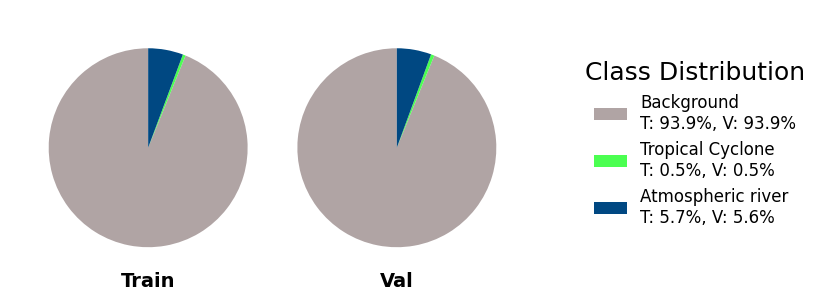
\includegraphics[width=1\textwidth]{graphics/background/data_distribution.png}
    \caption{Class Distribution}
    \label{fig:classdistribution}
\end{figure}


\begin{table}[h]
    \centering
    
    
    % Use p{width} for columns where you need wrapping text.
    \begin{tabular}{llccc}
        % \toprule
        \textbf{Type} & \textbf{Statistic} & \thead{\textbf{\#Masks} \\ \textbf{per Data Point}} & \thead{\textbf{Background/} \\ \textbf{Object } \\ \textbf{Per Mask}}  & \thead{\textbf{Background/} \\ \textbf{Object} \\ \textbf{per Data Point} } \\
        \midrule
        \multirow{2}{*}{\textbf{AR}}
            & Mean & 7.4 & 351.4 & 2,242 \\
            & Median & 7.0 & 142.2 & 17 \\
        \midrule
        \multirow{2}{*}{\textbf{TC}}
            & Mean & 2.6 & 880.7 & 149,220 \\
            & Median & 2.0 & 685.4 & 257 \\
        \bottomrule
    \end{tabular}
    \caption{Class Proportion and Object Statistics}
    \label{tab:summary_stats}
\end{table}






\subsection{Geographical Features and Constraint}
TCs are characterized by a distinct circular structure. Due to the lack of sufficient Coriolis force near the equator, these systems do not typically form within 5\degree{} of latitude. Instead, the vast majority of TCs originate within the latitudinal bands between 5\degree{} and 30\degree{} in both the Northern and Southern Hemispheres \cite{noaa_jetstream_tropical, hko_coriolis_tc}. Explainability analysis (LRP) confirms that CNNs indeed learn to look at point-shaped extrema in TMQ and circular wind motion to identify TCs \cite{radke2024explaining}.

ARs has narrow corridors or ``ribbons'' forms. These phenomena occur in both the Northern and Southern Hemispheres and are most commonly found in the mid-latitudes, typically between 30\degree{} and 60\degree{} \cite{gimeno2014atmospheric}. For AR detection, the models focus on elongated bands of high TMQ and eastward winds, which is physically plausible as ARs in both hemispheres are characterized by mid-latitude eastward moisture transport \cite{radke2024explaining}.

Consequently, when treating ClimateNet data points as spatial compositions, the geographic and geometric orientation of the corresponding labels is of critical importance. Because the formation of TCs and ARs are strictly governed by latitudinal physical constraints, the spatial context of these features is non-arbitrary. Therefore, standard geometric augmentation methods (e.g., vertical flipping or random rotations) should be avoided to ensure the model correctly learns the underlying geophysical semantics. Figure \ref{fig:world_projection_grid} illustrates four examples of data points from the ClimateNet dataset. As seen in these visualizations, the occurrence of these phenomena is variable; in some cases, TCs are not present within the provided time step, reflecting the natural distribution of extreme weather events.

% \begin{figure}[!h]
%     \centering
%     \begin{minipage}{0.48\textwidth}
%         \centering
%         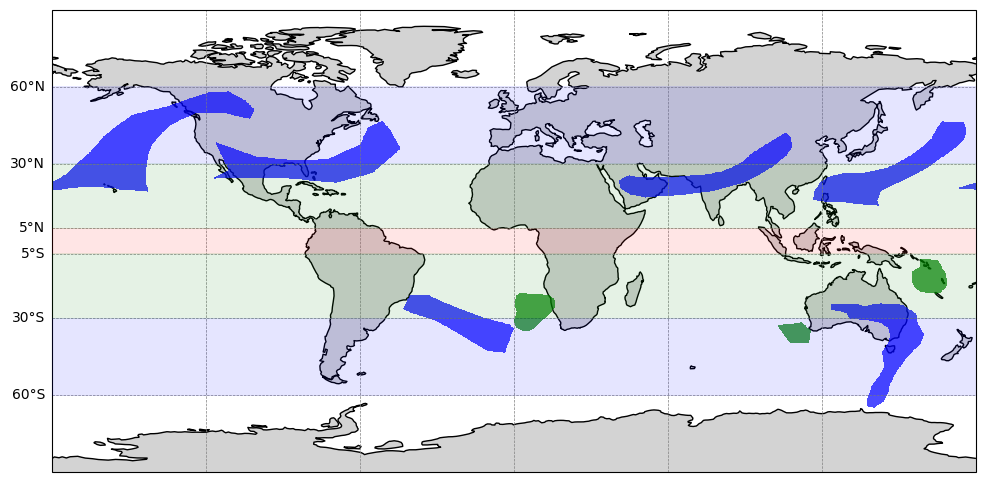
\includegraphics[width=1.05\textwidth]{graphics/background/data_example_1.png}
%         % \caption{a}
%     \end{minipage}
%     \hfill
%     \begin{minipage}{0.48\textwidth}
%         \centering
%         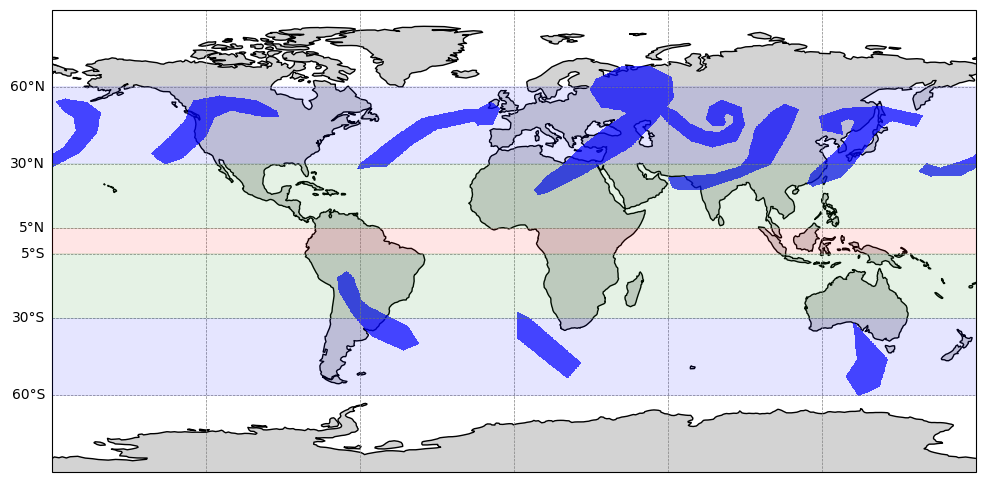
\includegraphics[width=1.05\textwidth]{graphics/background/data_example_2.png}
%         % \caption{b}
%     \end{minipage}
    
%     \vspace{0.5cm} % Add some vertical space
    
%     \begin{minipage}{0.48\textwidth}
%         \centering
%         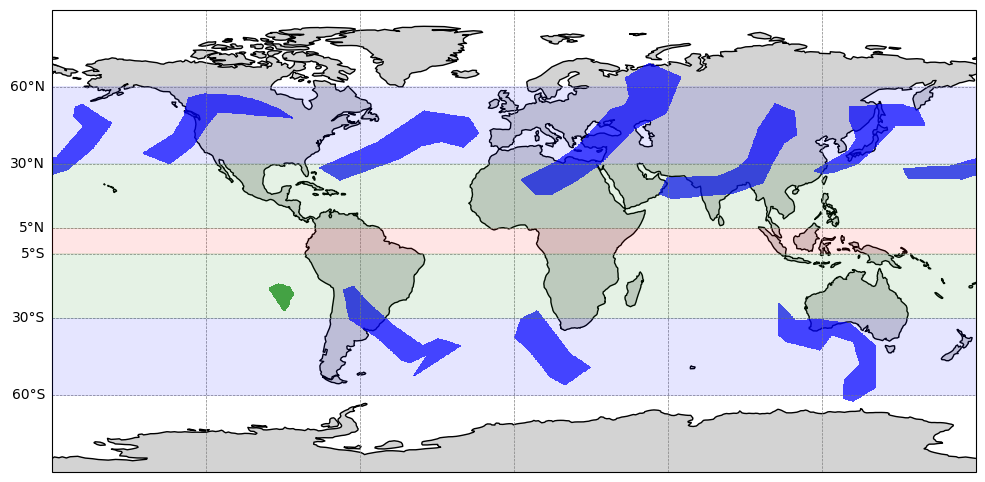
\includegraphics[width=1.05\textwidth]{graphics/background/data_example_3.png}
%         % \caption{c}
%     \end{minipage}
%     \hfill
%     \begin{minipage}{0.48\textwidth}
%         \centering
%         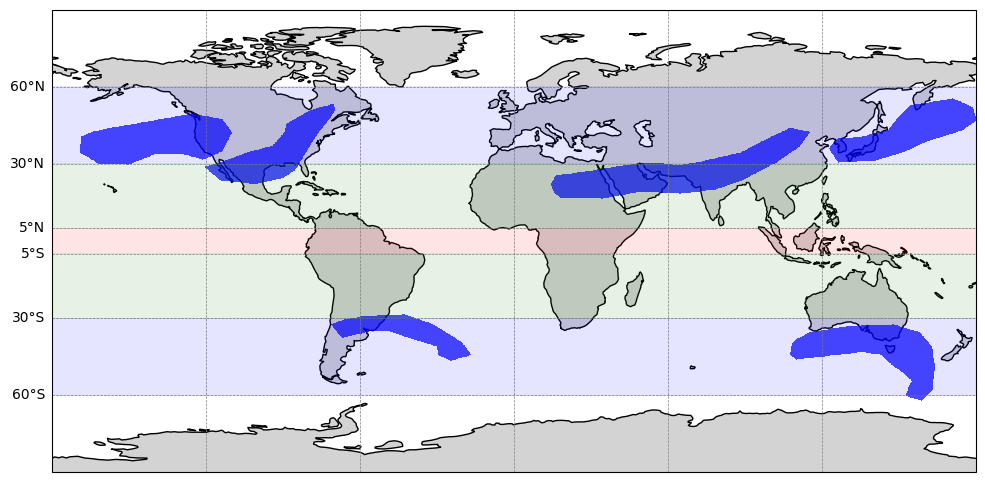
\includegraphics[width=1.05\textwidth]{graphics/background/data_example_4.png}
%         % \caption{d}
%     \end{minipage}
    
%     \caption{World projection visualizations of atmospheric data. The blue ``Ribons" are AR masks while, the green ones are TCs. The red band denotes the equatorial region between 5\degree{}N and 5\degree{}S where TCs do not typically form. The green bands (5\degree{} to 30\degree{} in both hemispheres) indicate the primary regions for TC activity. The purple bands (30\degree{} to 60\degree{} in both hemispheres) represent the mid\_latitudes where ARs typically occur.}
%     \label{fig:world_projection_grid}
% \end{figure}

\begin{figure}[!h]
    \centering
    \makebox[\textwidth][c]{%
        \begin{minipage}{1.0\textwidth}
            \centering
            \begin{minipage}{0.48\textwidth}
                \centering
                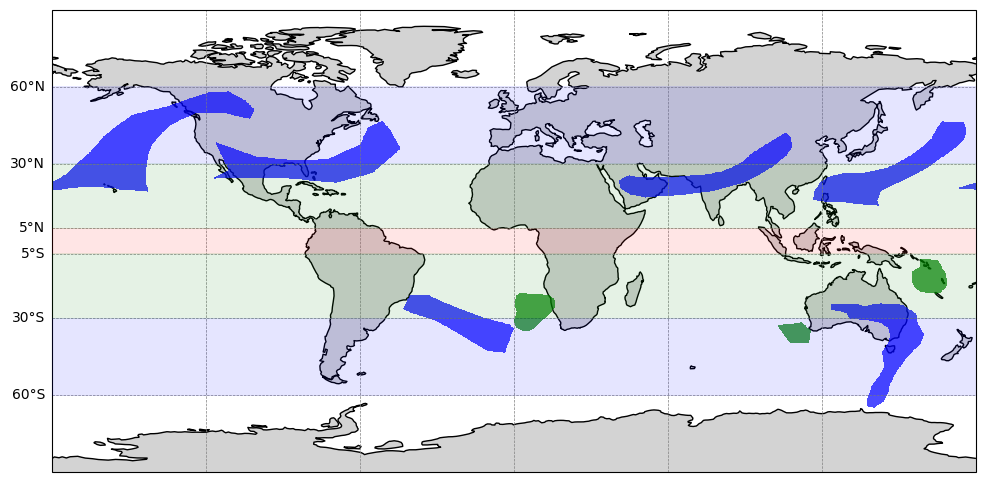
\includegraphics[width=1.05\textwidth]{graphics/background/data_example_1.png}
            \end{minipage}
            \hfill
            \begin{minipage}{0.48\textwidth}
                \centering
                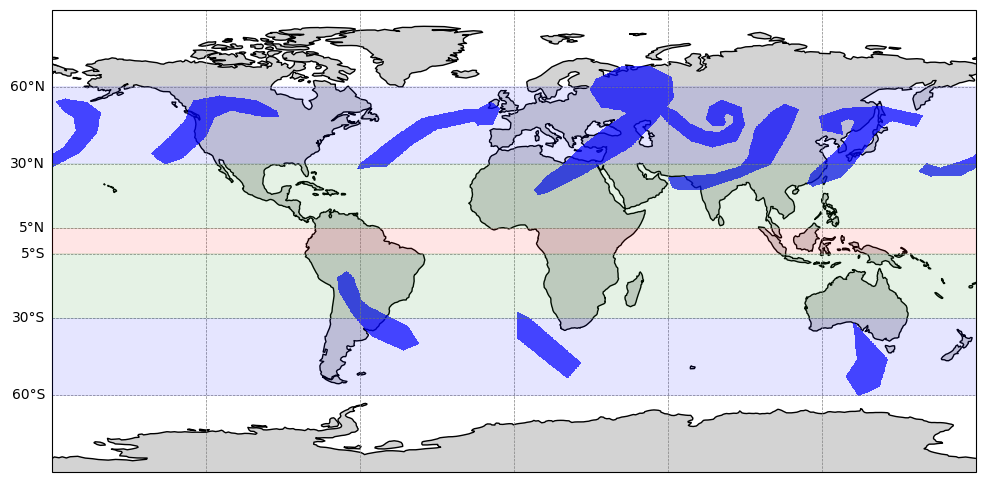
\includegraphics[width=1.05\textwidth]{graphics/background/data_example_2.png}
            \end{minipage}

            % \vspace{0.5cm}

            \begin{minipage}{0.48\textwidth}
                \centering
                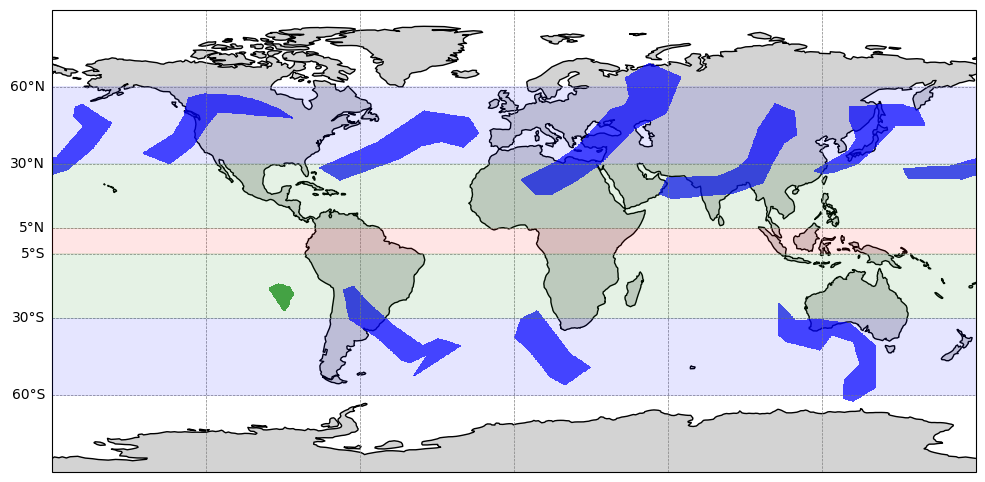
\includegraphics[width=1.05\textwidth]{graphics/background/data_example_3.png}
            \end{minipage}
            \hfill
            \begin{minipage}{0.48\textwidth}
                \centering
                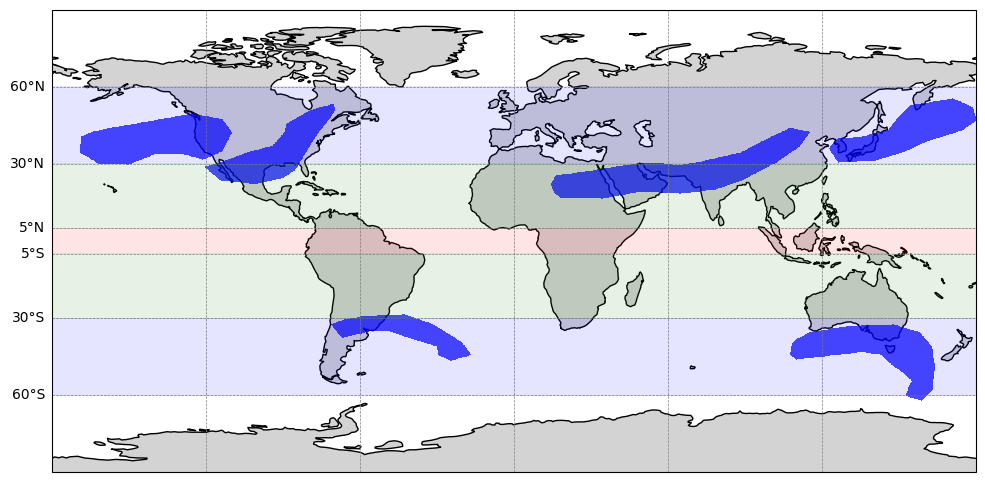
\includegraphics[width=1.05\textwidth]{graphics/background/data_example_4.png}
            \end{minipage}
        \end{minipage}
    }
    \caption{World projection visualizations of atmospheric data. The blue ``Ribons" are AR masks while, the green ones are TCs. The red band denotes the equatorial region between 5\degree{}N and 5\degree{}S where TCs do not typically form. The green bands (5\degree{} to 30\degree{} in both hemispheres) indicate the primary regions for TC activity. The purple bands (30\degree{} to 60\degree{} in both hemispheres) represent the mid\_latitudes where ARs typically occur.}
    \label{fig:data\_examples}
\end{figure}
SAM is a 2D guided model that requires a geometric prompt (or user prompt) to segment an image. The output is a set of segmentation masks at different levels and a confidence score for each. A segmentation mask is a 2D array with the same size as the image input. SAM consists of an encoder and a decoder. The encoder takes the image and geometric prompt to produce an image embedding, image position embedding, and geometric prompt embedding. The decoder takes in these various embeddings to produce segmentation masks and confidence scores.

\subsection{Geometric Prompts}
SAM supports three kinds of geometric prompts: points, bounding boxes, and dense masks. Points and bounding boxes are defined as sparse prompts, while dense masks are categorized as dense prompts.

\begin{itemize}
    \item A \textbf{point prompt} is a single pixel $(x, y)$. A positive point instructs the model to include the point in the produced segmentation mask, whereas a negative point instructs the model to exclude the pixel. The model accepts multiple points to guide the segmentation.
    
    \item A \textbf{bounding box} is defined by a top-left corner $(x_1, y_1)$ and a bottom-right corner $(x_2, y_2)$. Bounding boxes are always treated as positive prompts, instructing the model to produce the segment within the boxed area. Multiple bounding boxes may be provided.
    
    \item \textbf{Dense masks} are represented as a low-resolution 2D grid of size $256 \times 256 \times 1$. Each entry contains a floating-point value in the range $[0, 1]$, representing the probability that a pixel belongs to the segment mask.
\end{itemize}


\subsection{Prompt Embeddings}
\begin{figure}[!h]
    \centering
    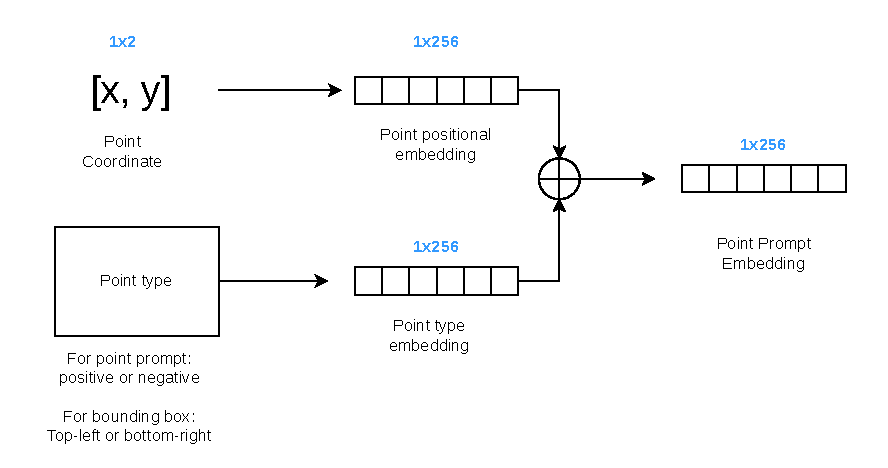
\includegraphics[width=1\textwidth]{graphics/background/point_embedding.pdf}
    \caption{Point Prompt Embedding}
    \label{fig:point_embedding}
\end{figure}


The PromptEncoder module in SAM maps geometric prompts to a latent space $\mathbb{R}^{256}$. Figure \ref{fig:point_embedding} illustrates the point prompt encoding process. It generates a positional encoding from spatial coordinates and a type embedding, each 
utilizing 256 trainable parameters. These vectors are combined via element-wise addition to produce the final 256-dimensional prompt embedding. All positive clicks use the same learned ``positive" vector, while negative clicks 
use a ``negative" vector. These 512 parameters are optimized during the training phase.

Similarly, bounding boxes are represented as a pair of point embeddings. To distinguish 
them from standard point prompts, SAM employs specific learned embeddings for the 
``top-left" and ``bottom-right" corners, resulting in two 256-dimensional vectors.

For the dense mask, the PromptEncoder downscales $256 \times 256 \times 1$ masks into dense embeddings 
of shape $256 \times 64 \times 64$, which are subsequently added element-wise to the 
image embeddings.

\subsection{Image Embeddings}
Figure \ref{fig:image_embedding} illustrates how SAM embed the image. The \texttt{ImageEncoderViT} accepts a raw input image, resizing it to a fixed resolution of $1024 \times 1024$. This input is processed into a $64 \times 64$ feature grid, creating a dense image embedding with a feature dimension of $256$. Within the \texttt{ImageEncoderViT}, various trainable parameters facilitate this transformation.

Simultaneously, the \texttt{PromptEncoder} generates positional embeddings for all $64 \times 64$ coordinates, resulting in an image positional embedding of shape $64 \times 64 \times 256$. The image content embedding tensor and its corresponding positional embedding are combined via element-wise addition to produce the final embedding. This final representation encapsulates both the semantic image 
information and the spatial positional information for all pixels. 

\begin{figure}[!h]
    \centering
    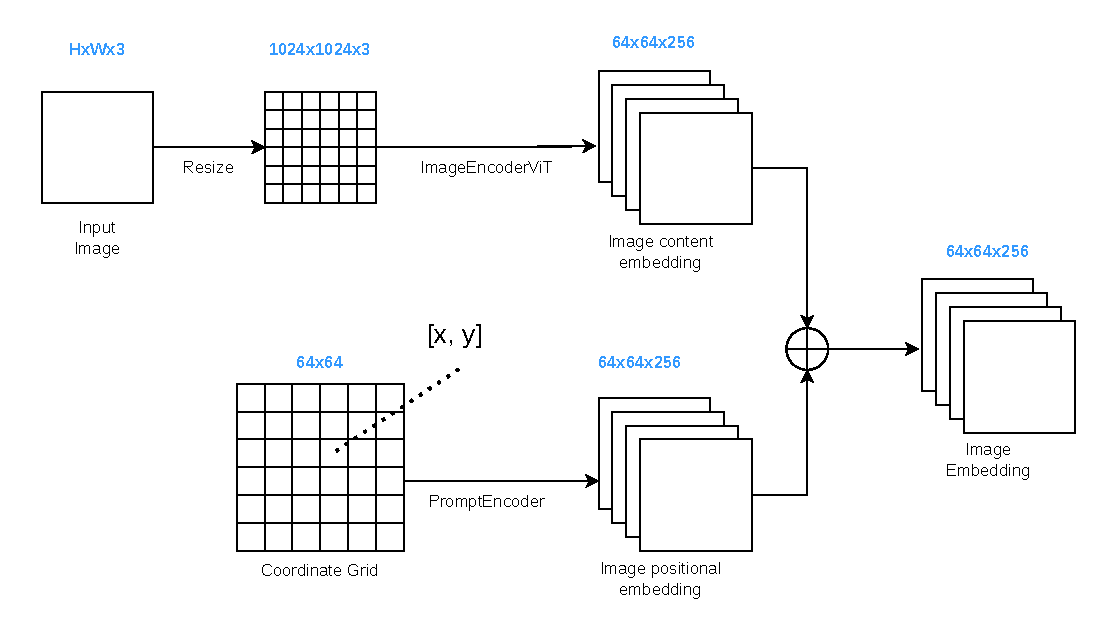
\includegraphics[width=1\textwidth]{graphics/background/image_embedding.pdf}
    \caption{Image Embedding}
    \label{fig:image_embedding}
\end{figure}

\subsection{Decoder}
The decoder inputs consist of the image positional embeddings, the image embedding, the dense mask embedding, and the sparse prompts. The image embedding and dense mask embedding are combined via element-wise addition to produce a $256 \times 64 \times 64$ tensor as input for the two-way transformer. The decoder also initializes a $1 \times 256$ IoU token and a $4 \times 256$ mask token from PyTorch's ``Embedding'' module. The figure \ref{fig:decoder} illustrates the decoding process.

The IoU token is not connected to any user input. During the transformer's processing, it is treated as an additional input along with the four mask tokens. It participates in the same two-way cross-attention layers, allowing it to attend to both the sparse prompt embeddings and the dense image features. This process enables the token to gather global context regarding how well the predicted mask aligns with the image data.

The four mask tokens serve as queries for the transformer. The attended mask tokens finally produce segmentation mask prediction heads for the four levels of masks. Three multi-mask tokens are designed for the ``subpart,'' ``part,'' and ``whole'' hierarchical levels, while the other token is optimized for unambiguous prompts, such as when a dense mask is already provided.

\begin{figure}[!h]
    \centering
    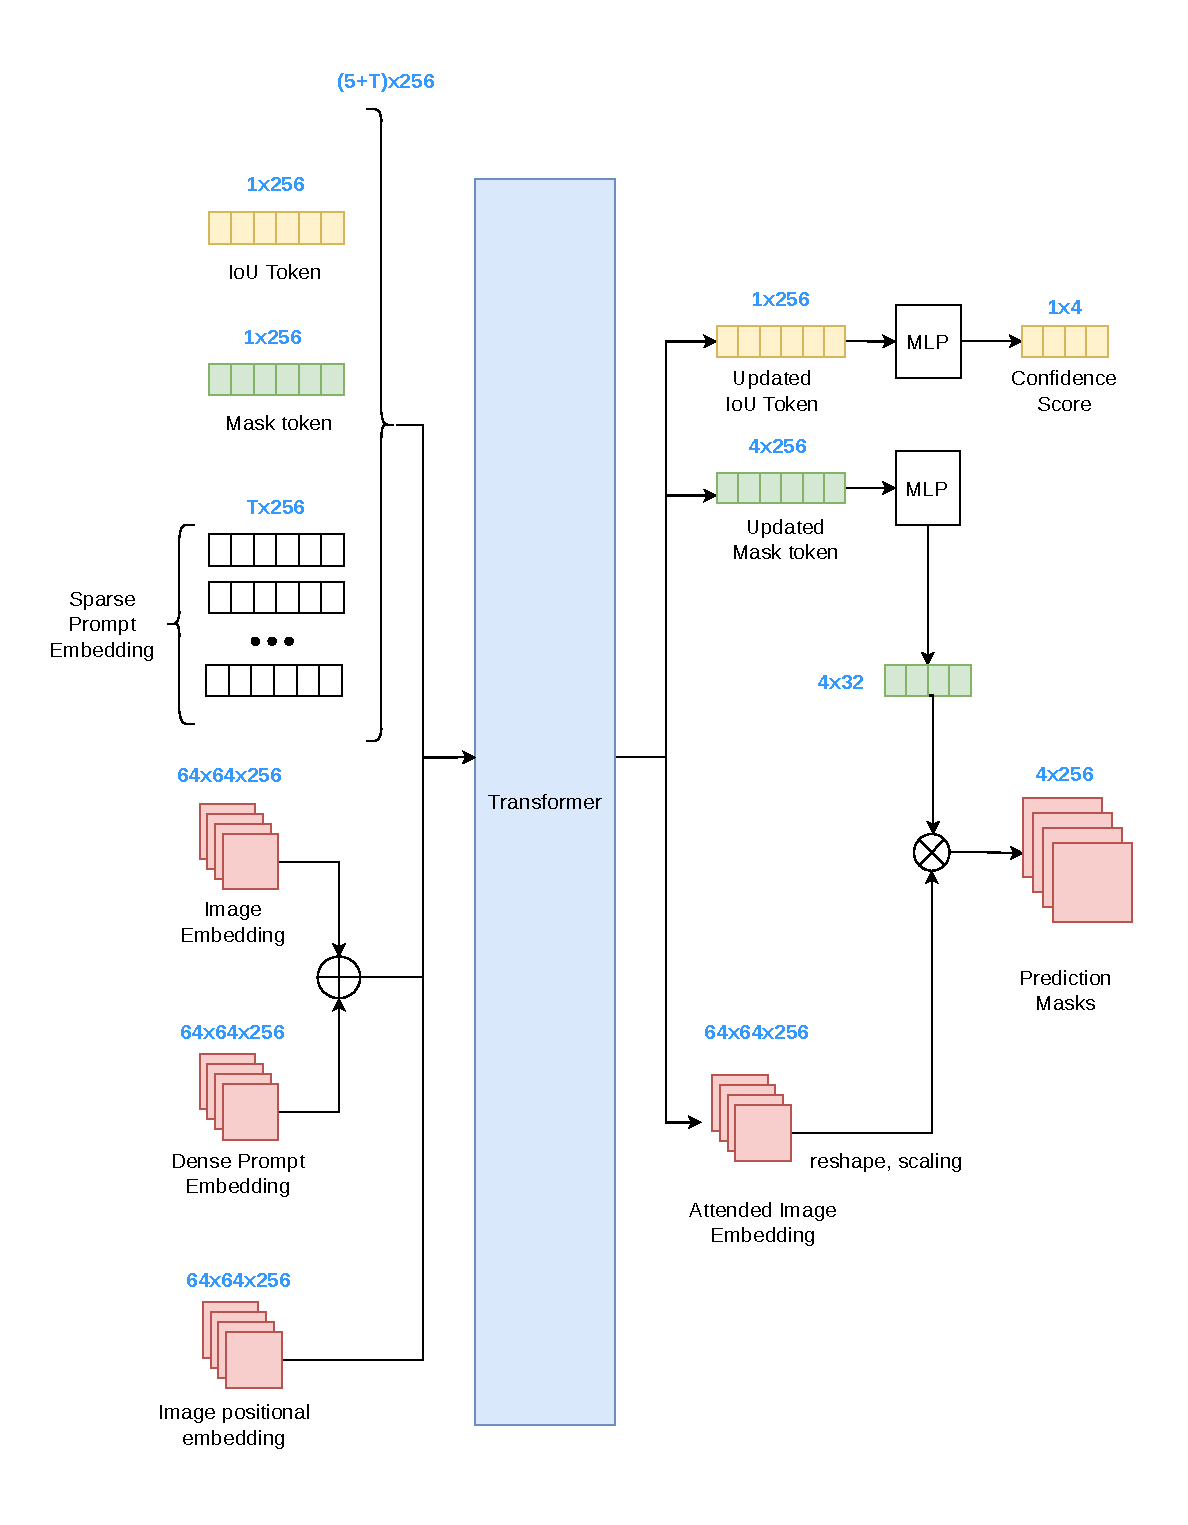
\includegraphics[width=1\textwidth]{graphics/background/decoder.pdf}
    \caption{Mask Decoder Process}
    \label{fig:decoder}
\end{figure}




\section{Parameter Efficient Fine-Tuning Techniques}
\subsection{LoRa}
To maintain the foundational knowledge of the pre-trained Segment Anything Model (SAM) while specializing it for meteorological features, we utilize Low-Rank Adaptation (LoRA)[cite: 341]. This approach is particularly effective for adapting SAM to the ClimateNet domain, as it allows for domain-specific refinement without the prohibitive computational cost of full parameter fine-tuning[cite: 301, 341].

\subsubsection{Conceptual Framework}
LoRA operates on the principle that the updates to the weights during adaptation have a low ``intrinsic rank". Instead of updating the massive original weight matrix $W$, we represent the update $\Delta W$ as the product of two much smaller, trainable matrices, $A$ and $B$. For a given input $x$, the modified forward pass is calculated as:

\begin{equation}
    y = Wx + \Delta Wx = Wx + BAx
\end{equation}

During the training phase, the original weight matrix $W$ remains frozen, and only the low-rank matrices $A$ and $B$ are updated. This significantly reduces the number of trainable parameters while allowing the model to capture the complex, non-image atmospheric patterns of Tropical Cyclones and Atmospheric Rivers.

\subsubsection{Implementation Details}
Our implementation focuses on injecting these adapters into the Transformer blocks of the SAM image encoder. Specifically, we target the Query ($q$) and Value ($v$) projection layers within the multi-head self-attention mechanism, as these layers are critical for internalizing the spatial relationships of weather phenomena.

\begin{itemize}
    \item \textbf{Rank Selection}: We utilize a small rank $r$ to ensure the adaptation remains efficient and prevents over-fitting to the sparse labels in the ClimateNet dataset.
    \item \textbf{Layer Injection}: Adapters are placed in parallel with the original linear layers, specifically targeting the $q$ and $v$ slices of the $qkv$ projection.
    \item \textbf{Initialization}: Matrix $A$ is initialized using a Kaiming uniform distribution to provide a stable starting gradient, while Matrix $B$ is initialized to zero. This ensures that at the beginning of training, the "shortcut" has zero impact, and the model starts with the exact behavior of the vanilla SAM.
\end{itemize}

\subsubsection{Strategic Advantages}
By employing LoRA, we isolate the adaptation process of the encoder[cite: 343]. This methodology ensures that the model focuses exclusively on learning to extract high-quality, diagnostic features from the 16 multi-parameter atmospheric grids[cite: 344]. This is vital for recognizing the "ribbon-like" corridors of ARs and the "circular" structures of TCs, which differ significantly from the high-frequency edges found in traditional RGB images[cite: 345].

\subsection{Learnable Token}
In CAT-SAM-T and HQ-SAM, a small learnable token of dimension 1×256 is introduced \cite{xiao2024cat, ke2023segment}. This token is combined via element-wise addition with the original IoU token embedding to initialize a refined IoU token. Following processing through the transformer blocks, the updated token incorporates global image context, critical geometric and categorical information from the prompt tokens, and latent mask information from other output tokens. The refined token is then passed through an MLP and subsequently undergoes a spatially point-wise product with the fused image features to facilitate high-quality mask generation.

\subsection{Loss Functions}

In the ClimateNet dataset, a significant challenge arises from the extreme class imbalance. Background pixels constitute approximately \textbf{93.9\%} of the data, while Atmospheric Rivers (ARs) represent \textbf{5.7\%} and Tropical Cyclones (TCs) represent only \textbf{0.5\%} \cite{56, 68}. Furthermore, TCs are substantially rarer and smaller than ARs, with an average of only \textbf{2.6} TC masks per image compared to \textbf{7.4} for ARs \cite{54, 76}. The ratio of background area to TC area is particularly skewed at \textbf{257:1} \cite{56, 76}. 

To effectively tackle these disparities and the ``ribbon-like" or ``circular" structures of these phenomena, a well-designed loss function is required \cite{72, 255}. Originally, SAM utilized a hybrid approach combining Focal Loss and Dice Loss to balance pixel-level classification with regional overlap \cite{166}.

\subsubsection{Focal Loss}
Standard Cross-Entropy loss often fails when foreground objects are proportionally much smaller than the background, as the model can achieve high accuracy by simply predicting the majority class. Focal Loss addresses this by adding a modulating factor to the standard criterion to focus on ``hard" examples \cite{166}.

\begin{equation}
L_{focal} = -\alpha_t (1 - p_t)^\gamma \log(p_t)
\end{equation}

\begin{itemize}
    \item $p_t$: Represents the model's estimated probability for the ground truth class \cite{166}. 
    \item $\gamma$: The focusing parameter. When $\gamma = 0$, Focal Loss is equivalent to Cross-Entropy. As $\gamma$ increases, the loss for ``easy" examples is down-weighted \cite{166}.
    \item $(1 - p_t)^\gamma$: The modulating factor. It reduces the loss contribution from easy pixels, forcing the model to concentrate on ambiguous pixels typically found at the boundaries of TCs and ARs \cite{166}.
    \item $\alpha_t$: A balancing parameter used to handle the prior probability of classes, providing a baseline weight to the rare TC and AR pixels \cite{166}.
\end{itemize}

The modulating factor $(1-p_t)^\gamma$ acts as a dynamic weight that determines which outcomes contribute most to the gradient:
\begin{equation}
L_{focal} = 
\begin{cases} 
-\alpha (1 - p)^\gamma \log(p) & \text{if } y=1 \text{ (Focuses on False Negatives)} \\
-(1 - \alpha) p^\gamma \log(1 - p) & \text{if } y=0 \text{ (Focuses on False Positives)} 
\end{cases}
\end{equation}
\begin{itemize}
    \item Easy TP: When $y=1$ (ground truth = 1) and $p \to 1$, $(1-p)^\gamma$ approaches 0, effectively ``muting" pixels the model is already confident about \cite{166}.
    \item Hard FN: When $y=1$ but $p \to 0$ (a missed detection), $(1-p)^\gamma$ remains near 1, keeping the loss signal high to force the model to identify the missed TC or AR \cite{166, 255}.
    \item Easy TN: When $y=0$ and $p \to 0$, $p^\gamma$ becomes very small. This prevents the 93.9\% of background pixels from overwhelming the gradient \cite{68, 166}.
    \item Hard FP: When $y=0$ but $p \to 1$ (a false alarm), $p^\gamma$ stays high to penalize over-segmentation in clear atmospheric regions \cite{166}.
\end{itemize}

\subsubsection{Dice Loss}
While Focal Loss operates at the individual pixel level, Dice Loss evaluates the global overlap between the predicted mask and the ground truth. To better understand its relationship with classification metrics, it can be expressed in terms of True Positives (TP), False Positives (FP), and False Negatives (FN).

\begin{equation}
L_{dice} = 1 - \frac{2|A \cap B|}{|A| + |B|} = 1 - \frac{2TP}{2TP + FP + FN}
\end{equation}

\begin{itemize}
    \item $A$: The set of predicted pixels for the mask.
    \item $B$: The set of ground truth pixels.
    \item $TP$: True Positives; pixels correctly identified as part of the TC or AR.
    \item $FP$: False Positives; the over-segmentation pixels.
    \item $FN$: False Negatives; the missed detection pixels.
\end{itemize}

Dice Loss is scale-invariant. Because it normalizes the intersection by total pixels, a small error on a tiny TC mask is penalized as heavily as an error on a large AR mask \cite{166}. However, standard Dice Loss treats FP and FN with equal importance, which may not be ideal for meteorological applications where missing a rare TC (a False Negative) is often more critical than a slight over-estimation of its boundary. This limitation leads to the introduction of a more flexible framework: the Tversky Loss.

\subsubsection{Tversky Loss}
The Tversky Index (TI) is a generalization of the Dice coefficient that allows for asymmetrical weighting of False Positives and False Negatives.

\begin{equation}
L_{Tversky} = 1 - \frac{TP}{TP + \alpha FP + \beta FN}
\end{equation}

\begin{itemize}
    \item $\alpha$: The weight assigned to False Positives. Increasing $\alpha$ improves precision by penalizing predicted pixels that do not belong to the ground truth.
    \item $\beta$: The weight assigned to False Negatives. Increasing $\beta$ improves recall (sensitivity) by penalizing the model for missing ground truth pixels.
\end{itemize}
If $\alpha = \beta = 0.5$, the function simplifies to the Dice Loss. If $\alpha = \beta = 1.0$, it simplifies to the Jaccard Index (IoU).

\subsubsection{Hybrid Loss Functions}
Modern segmentation adaptations, such as CAT-SAM \cite{389} and HQ-SAM \cite{383}, frequently employ hybrid loss strategies to leverage the strengths of both distribution-based and region-based functions \cite{162, 383, 389}. While the original SAM architecture focuses on a linear combination of Focal and Dice losses for general-purpose segmentation, domain-specific adaptations often swap Dice for Tversky to handle high-stakes sensitivity requirements \cite{166, 389}.

In this study, we use the combination of Tversky and Focal Loss for adapting SAM to the ClimateNet domain. While the Tversky component ensures the model captures the full extent of weather features by prioritizing recall through $\beta$, the Focal component ensures the model classifies difficult boundary pixels that are otherwise lost in the massive background grid \cite{207, 255}. This hybrid approach effectively mitigates the challenges posed by the extreme background-to-TC ratio \cite{56}.

\chapter{Approach}
While the Segment Anything Model (SAM) has demonstrated remarkable zero-shot generalization in the computer vision domain, its application to meteorological data presents two fundamental challenges. First, SAM is inherently designed for three-channel RGB images, whereas climate data, such as the ClimateNet dataset, consists of multi-parameter atmospheric grids. Unlike natural images, these variables lack high-frequency edges and clear semantic boundaries, making the standard image encoder less effective at capturing the underlying geophysical features.

Second, the operational utility of SAM is limited by its reliance on manual geometric prompts (points, boxes, or masks) to guide segmentation. In a real-time meteorological forecasting context, requiring a human expert to provide manual prompts for every global raster is impractical. Therefore, our objective is to transition SAM toward a prompt-free architecture capable of autonomous detection.

To achieve a prompt-free system that remains grounded in the physical realities of the dataset, we divide our approach into two distinct phases, as illustrated in Figure \ref{fig:pipeline}. In the Adaptation Phase, we experiment with a learnable token-based approach, inspired by HQ-SAM \cite{ke2023segment} and CAT-SAM-T \cite{xiao2024cat}, as well as a LoRA-based approach, inspired by LoRA-SAM \cite{zhang2024improving}. In the Prompt Generation Phase, we first use a pretrained CGNet from ClimateNet to produce auxiliary masks. We also experiment with a multi-scale fusion module, inspired by Self-Prompt SAM \cite{xie2025self}.

% \begin{figure}[!h]
%     \centering
%     \includegraphics[width=0.8\textwidth]{graphics/approach/approach_pipeline.pdf}
%     \caption{Pipeline}
%     \label{fig:pipeline}
% \end{figure}

\begin{figure}[!h]
    \centering
    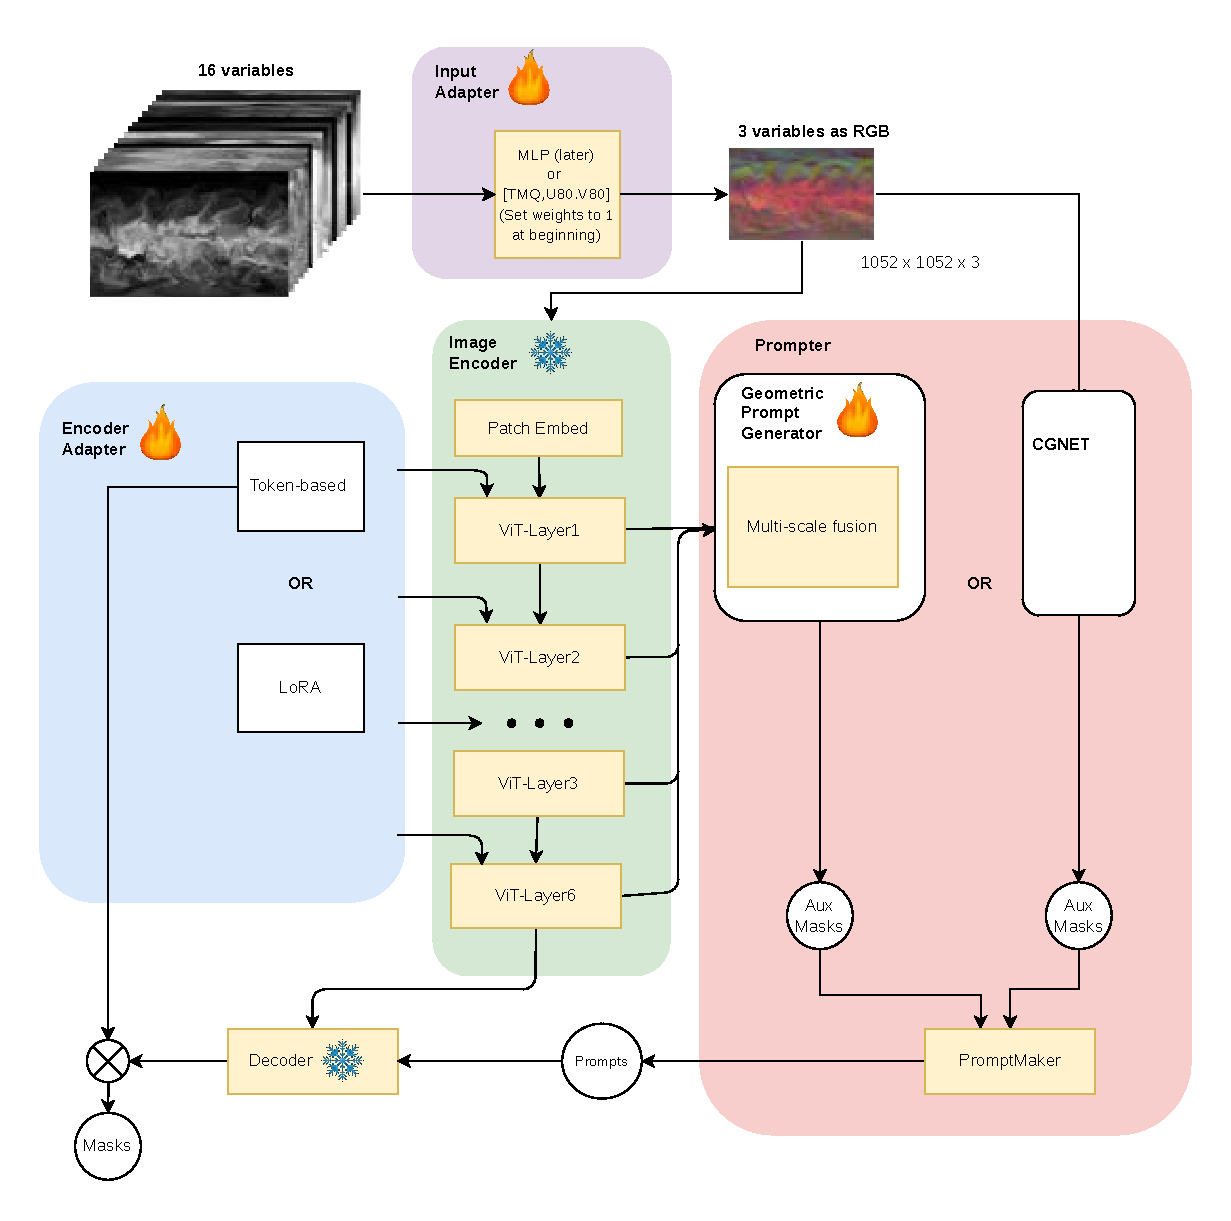
\includegraphics[width=1\textwidth]{graphics/approach/pipeline.pdf}
    \caption{Experiment Pipeline}
    \label{fig:pipeline}
\end{figure}

\subsubsection{Phase 1: Adaptation and Encoder Refinement}

The primary objective of the first phase is to enable the SAM  to interpret non-image atmospheric variables, which differ significantly from the RGB data for which the model was originally optimized. To bridge the structural gap between the 16 multi-channel atmospheric grids  and the fixed input requirements of the SAM image encoder, we implement a dual adaptation strategy:

\begin{enumerate}
\item Learnable Token-based Adaptation: We introduce learnable tokens to compress the high-dimensional atmospheric channels into a latent representation that aligns with the encoder's expected feature space.
\item Low-Rank Adaptation (LoRA): To maintain the foundational knowledge of the pre-trained model while specializing it for meteorological features, we utilize LoRA to fine-tune specific layers within the encoder and mask decoder.
\end{enumerate}


During this stage, the model is trained under the assumption of ``perfect prompts". By providing the system with ground-truth bounding boxes or point coordinates during the training phase , we isolate the adaptation process of the encoder and the mask decoder. This methodology ensures that the model focuses exclusively on learning to extract high-quality, diagnostic features from critical variables.

By removing the variability of prompt quality, we can more accurately evaluate the model's ability to handle the ``ribbon-like" structures of Atmospheric Rivers (ARs) and the circular patterns of Tropical Cyclones (TCs) , effectively mitigating the challenges posed by data imbalance and the lack of traditional image-style boundaries.

\subsubsection{Phase 2: Automated Prompt Generation}
Once the encoder is successfully adapted to the ClimateNet domain, we introduce a generator module to eliminate the need for manual intervention. This generator leverages the embeddings produced by the encoder to automatically predict the locations of TCs and ARs. By treating the image embeddings as a rich source of contextual information, the generator produces auxiliary segmentation masks. These masks are then processed to generate point and bounding box prompts, which are fed into the mask decoder to produce the final segmentation for evaluation.

\section{Dataset Preparation}
% Here I would write how the data from sources, z-normalize, make it images again by multiply by 255. 
% How prompts is make, take the multimask ground truth, find connected component, filter out, get N positive points, or M negative points per object masks, bounding box, noisy mask (resize, iroduce noise, 

The Figure \ref{fig:prompt_pipeline} illustrates the overall pipeline of prompt preparation for GAN. This includes creating point prompts, bounding box prompts, and noisy mask prompts for the input adapter in phase 1 as well as creating prompts from auxiliary masks from automatic prompt generator from phase 3.

\begin{figure}[!h]
    \centering
    % 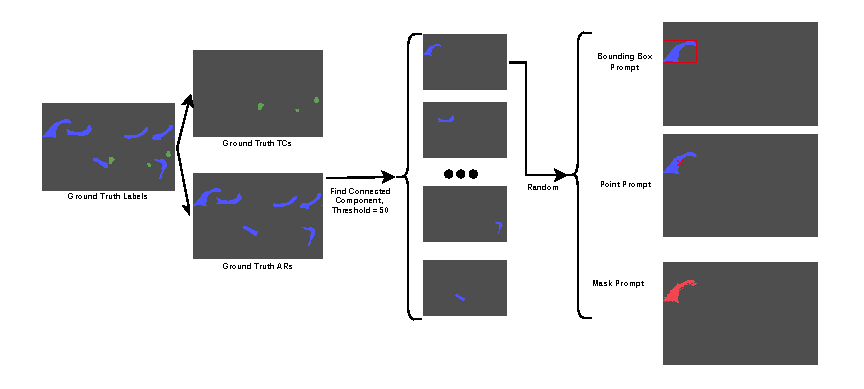
\includegraphics[width=1\textwidth]{graphics/approach/prompt_pipeline-1.pdf}
    \makebox[\textwidth][c]{%
    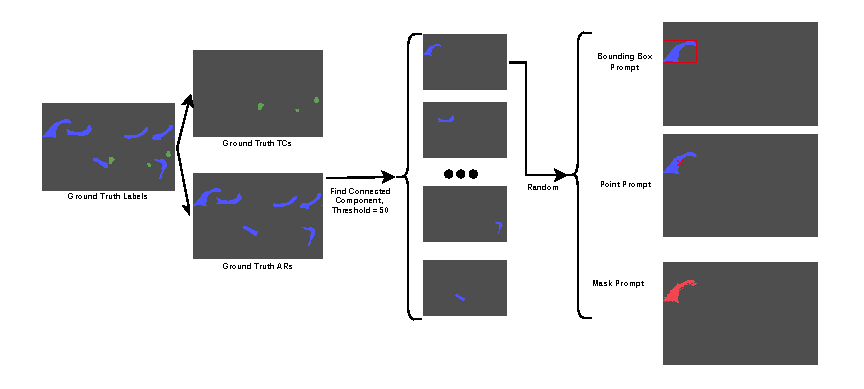
\includegraphics[width=1.2\textwidth]{graphics/approach/prompt_pipeline-1.pdf}
}
    \caption{Prompt Preparation Process}
    \label{fig:prompt_pipeline}
\end{figure}

The Figure \ref{fig:point_prompt_generation} and \ref{fig:noisy_mask_generation} describe the process of creating point prompts and noisy mask prompts in detail. To generate positive point prompts, the binary mask is first processed using an erosion operation with a kernel size determined by the object area. Positive points are then randomly sampled from this eroded region, ensuring the points remain well within the object boundaries. For negative point prompts, the pipeline utilizes two different dilation kernels. A smaller kernel and a big kernel are applied to the mask, and the smaller dilated version is subtracted from the larger one to define a boundary region for sampling negative points. 

\vspace{-2em}
\begin{figure}[!h]
    \centering
    % 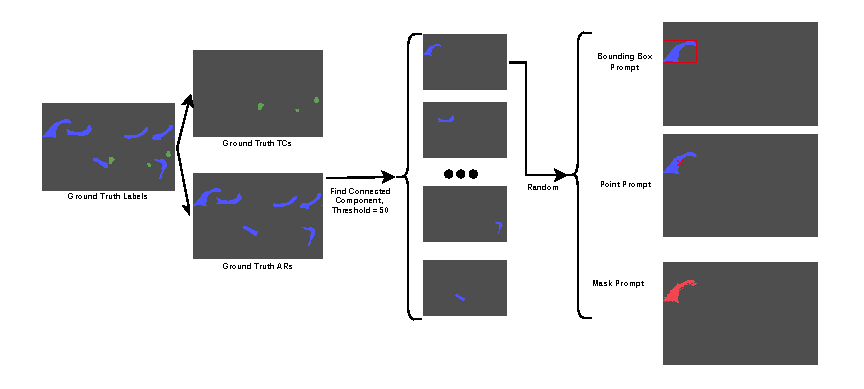
\includegraphics[width=1\textwidth]{graphics/approach/prompt_pipeline-1.pdf}
    \makebox[\textwidth][c]{%
    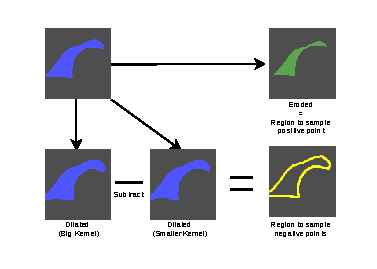
\includegraphics[width=0.7\textwidth]{graphics/approach/point_prompt.pdf}
}
\vspace{-2em}
    \caption{Sampling Negative and Positive Point Prompts}
    \label{fig:point_prompt_generation}
\end{figure}

The noisy mask prompt generation involves a multi-step interpolation and residue calculation process. The input mask is interpolated to a small size and then interpolated back to its original size to create a recovered mask. This recovered version is subtracted from the original input to identify incoherent regions. These regions are thresholded and then combined with Gaussian noise via element\_wise multiplication. Finally, the noise is integrated back into the mask through element\_wise addition to produce a dense, noisy mask prompt.

\vspace{-2em}
\begin{figure}[!h]
    \centering
    % 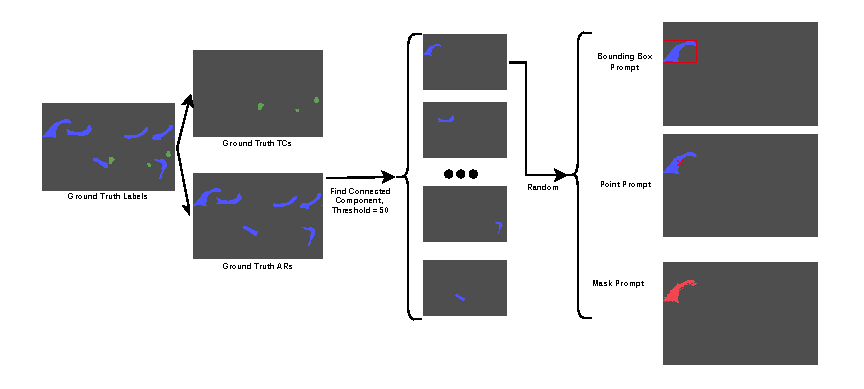
\includegraphics[width=1\textwidth]{graphics/approach/prompt_pipeline-1.pdf}
    \makebox[\textwidth][c]{%
    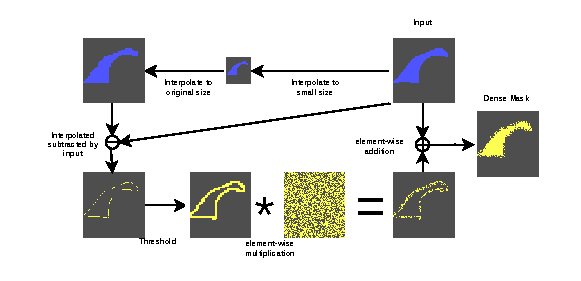
\includegraphics[width=1.2\textwidth]{graphics/approach/noisy_mask.pdf}
}
\vspace{-2em}
    \caption{Create Noisy Mask Prompts}
    \label{fig:noisy_mask_generation}
\end{figure}


% \begin{figure}[!h]
% \centering
% \vspace{-3em} 
% % Top Image
% % \begin{center}
% %     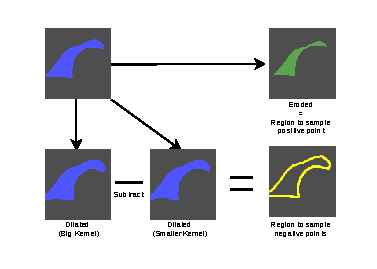
\includegraphics[width=0.7\textwidth]{graphics/approach/point_prompt.pdf}
% %     \caption{Sampling Negative and Positive Point Prompts}
% %     \label{fig:point_prompt_generation}
% % \end{center}
% \vspace{-3em} % Adds a small vertical gap between the two plots
% % Bottom Image
% \begin{center}
%     % \makebox[\textwidth][c]{%
%     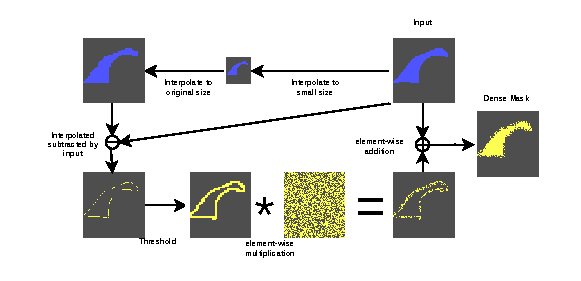
\includegraphics[width=1\textwidth]{graphics/approach/noisy_mask.pdf}
%     \caption{Create Noisy Mask Prompts}
%     \label{fig:noisy_mask_generation}
% \end{center}

% \caption{Prompt Generating Process}


% \end{figure}
\section{Architectures}
\label{sec:architectures}

This section describes the various architectural components utilized in the development of ClimateSAM. To adapt the SAM for ClimateNet Dataset, the framework incorporates specialized modules for data adaptation, feature refinement, and autonomous guidance. The overall architecture, as visualized in Figure \ref{fig:pipeline}, is designed to handle the 16-channel atmospheric grids of ClimateNet while transitioning SAM toward a prompt-free operational state.

The system comprises three main architectural pillars:
\begin{itemize}
    \item \textbf{Input Adapter}: A newly suggested ClimateInputAdapter is implemented as a learnable bottleneck convolutional module. It compresses the high-dimensional atmospheric data into a 3-channel pseudo-RGB representation, ensuring compatibility with the SAM image encoder while preserving critical physical signals.
    \item \textbf{Encoder Adapters}: Two Parameter-Efficient Fine-Tuning (PEFT) strategies are explored to adapt the frozen ViT backbone. These include a \textit{learnable token-based} mechanism to steer the model using latent representations and a \textit{LoRA-based} approach that utilizes low-rank matrix decomposition to update the query and value projections.
    \item \textbf{Prompt Generators}: To achieve autonomous detection, the pipeline evaluates two prompter architectures. We utilize \textit{CGNet} an established lightweight convolutional network for semantic segmentation alongside a newly introduced \textit{Multi-scale Fusion Module}. This module leverages intermediate encoder features to generate auxiliary masks, which are then converted into sparse geometric prompts for the mask decoder.
\end{itemize}



\subsection{Input Adapter}
The ClimateInputAdapter is a specialized learnable preprocessing module designed to bridge the structural gap between multi-parameter atmospheric grids and the fixed input requirements of the Segment Anything Model (SAM). Since SAM is natively optimized for three-channel RGB imagery, this adapter compresses the 16 atmospheric variables from the ClimateNet dataset into a pseudo-RGB representation that preserves critical geophysical features. 

As depicted in Figure \ref{fig:input_adapter}, the architecture follows a bottleneck convolutional design. It initiates with a 3x3 Conv2d layer to capture local spatial dependencies, followed by sequential 1x1 convolutions that reduce the feature dimensionality from 32 to 16, and ultimately to 3 channels. The module incorporates BatchNorm2d and ReLU activations for internal stabilization. A final Sigmoid activation function constrains the output values to a [0, 1] range, which are subsequently rescaled by 255.0 to align with the standard pixel intensity expected by the SAM image encoder.
\vspace{-1em}
\begin{figure}[!h]
    \centering
    % 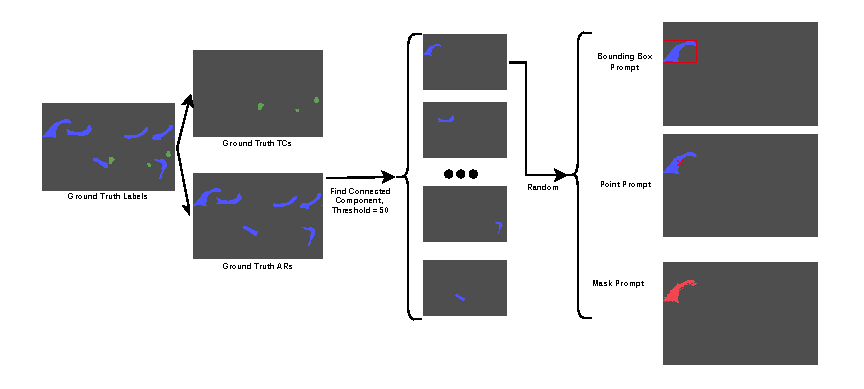
\includegraphics[width=1\textwidth]{graphics/approach/prompt_pipeline-1.pdf}
    \makebox[\textwidth][c]{%
    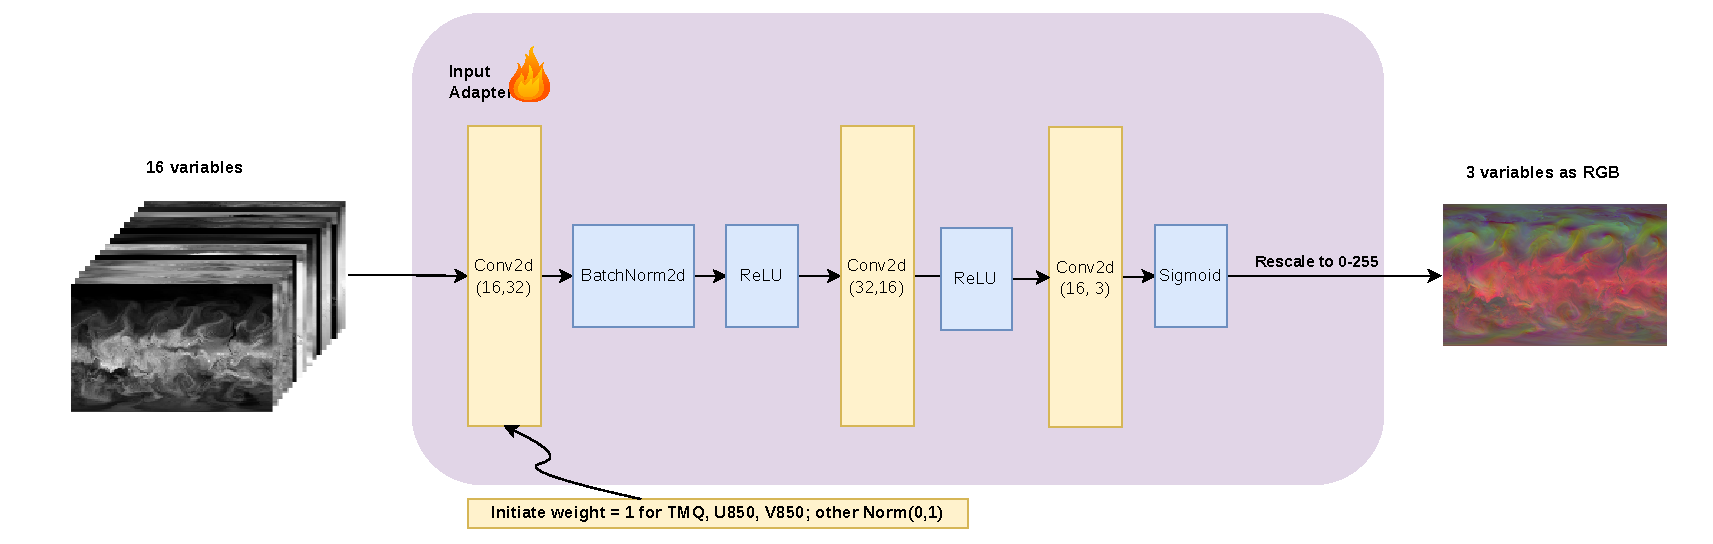
\includegraphics[width=1.3\textwidth]{graphics/approach/input_adapter.pdf}
}
\vspace{-1em}
    \caption{Input Adapter Architecture}
    \label{fig:input_adapter}
\end{figure}


To maintain physical grounding during the Adaptation Phase, the adapter employs an expert-knowledge initialization strategy. The weights for the most diagnostic variables TMQ, U850, V850, and PSL \cite{radke2024explaining} are set to 1.0 at the center of the convolution kernels. This initialization enables the model to prioritize the point-shaped extrema characteristic of Tropical Cyclones and the elongated moisture corridors of Atmospheric Rivers from the onset of training.
\subsection{Encoder Adapter}

\subsubsection{Learnable Token-based approach}

\begin{figure}[!h]
    \centering
    \begin{minipage}[b]{0.45\textwidth}
        \centering
        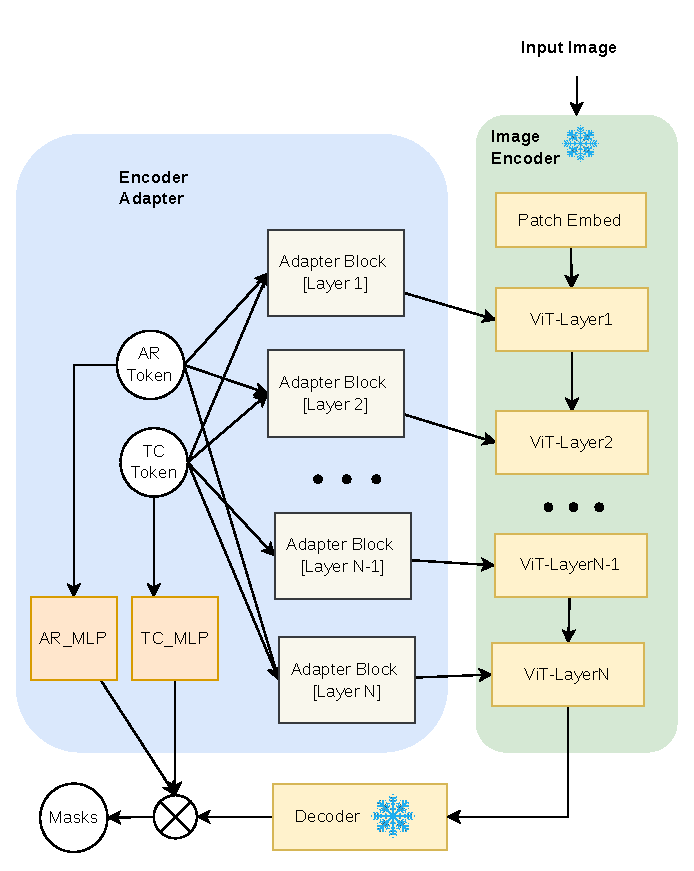
\includegraphics[width=\textwidth]{graphics/approach/token_based_overview.pdf}
        \caption{Overview}
    \end{minipage}
    \hfill
    \begin{minipage}[b]{0.45\textwidth}
        \centering
        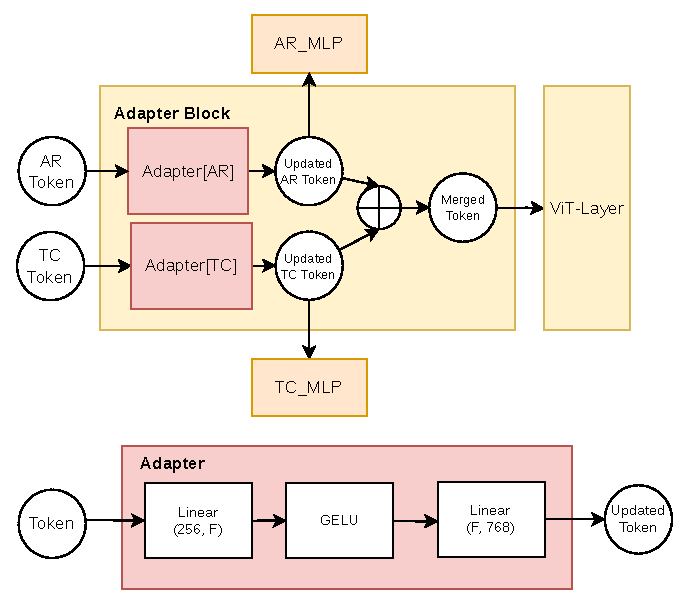
\includegraphics[width=\textwidth]{graphics/approach/token_based_detail.pdf}
        \caption{Detail}
    \end{minipage}
    \caption{Token-based approach architecture}
    \label{fig:token_architecture}
\end{figure}

\subsubsection{LoRA approach}
To adapt SAM to interpret multi-parameter atmospheric grids, we apply LoRA adapters to each layer of the Vision Transformer (ViT) encoder \cite{wu2025multi, zhang2024improving}. This "surgeon" approach specifically targets the Query ($q$), Key ($k$), and Value ($v$) projection layers within the multi-head self-attention mechanism, as these layers are critical for capturing the spatial relationships of complex weather phenomena. Mathematically, for an input feature $x \in \mathbb{R}^{1 \times d}$, the adapted forward pass for a given projection is expressed as:
\begin{equation}
h = W_{0}x + \Delta Wx = W_{0}x + BAx
\end{equation}
where $W_0$ is the frozen pre-trained weight, and $B \in \mathbb{R}^{d \times r}$ and $A \in \mathbb{R}^{r \times d}$ are the learnable low-rank matrices \cite{zhu2024melo, wu2025multi}. We initialize matrix $A$ with a Kaiming uniform distribution and matrix $B$ to zero so that the initial state of the model is identical to the original SAM. At the output stage, we introduce two specialized mask decoders with learnable parameters to handle the distinct morphological characteristics of the target classes:

\begin{itemize}
    \item \textbf{TC Decoder}: Optimized for the distinct circular structures of Tropical Cyclones, addressing a severe 257:1 background-to-foreground ratio.
    \item \textbf{AR Decoder}: Tailored for the narrow, "ribbon-like" corridors of Atmospheric Rivers, which present a more moderate 17:1 class imbalance.
\end{itemize}

This dual-decoder design allows the model to learn class-specific localization priors and structural discovery independently for each meteorological feature.

% \ifdefined\pdfobjcompresslevel
%   \pdfobjcompresslevel=0
% \fi
% \ifdefined\pdfvariable
%   \pdfvariable objcompresslevel=0
% \fi

\begin{figure}[!h]
    \centering
    \begin{minipage}[b]{0.5\textwidth}
        \centering
        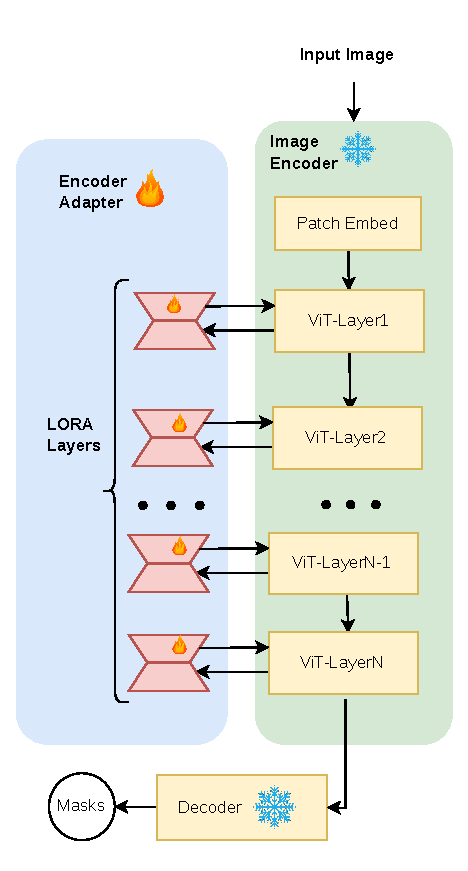
\includegraphics[width=\textwidth]{graphics/approach/lora_overview.pdf}
        \caption{Overview}
    \end{minipage}
    \hfill
    \begin{minipage}[b]{0.45\textwidth}
        \centering
        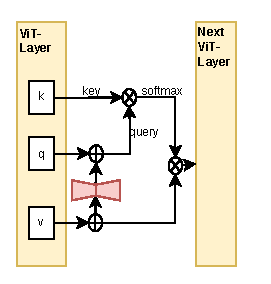
\includegraphics[width=\textwidth]{graphics/approach/lora_detail.pdf}
        \caption{Detail}
    \end{minipage}
    \caption{LoRA adaptation architecture}
    \label{fig:lora_architecture}
\end{figure}

\subsection{Automatic Prompt Generator}

\subsubsection{CGNet}

\subsubsection{Multi-scale Fusion}

\begin{figure}[!h]
    \centering
    \makebox[\textwidth][c]{%
        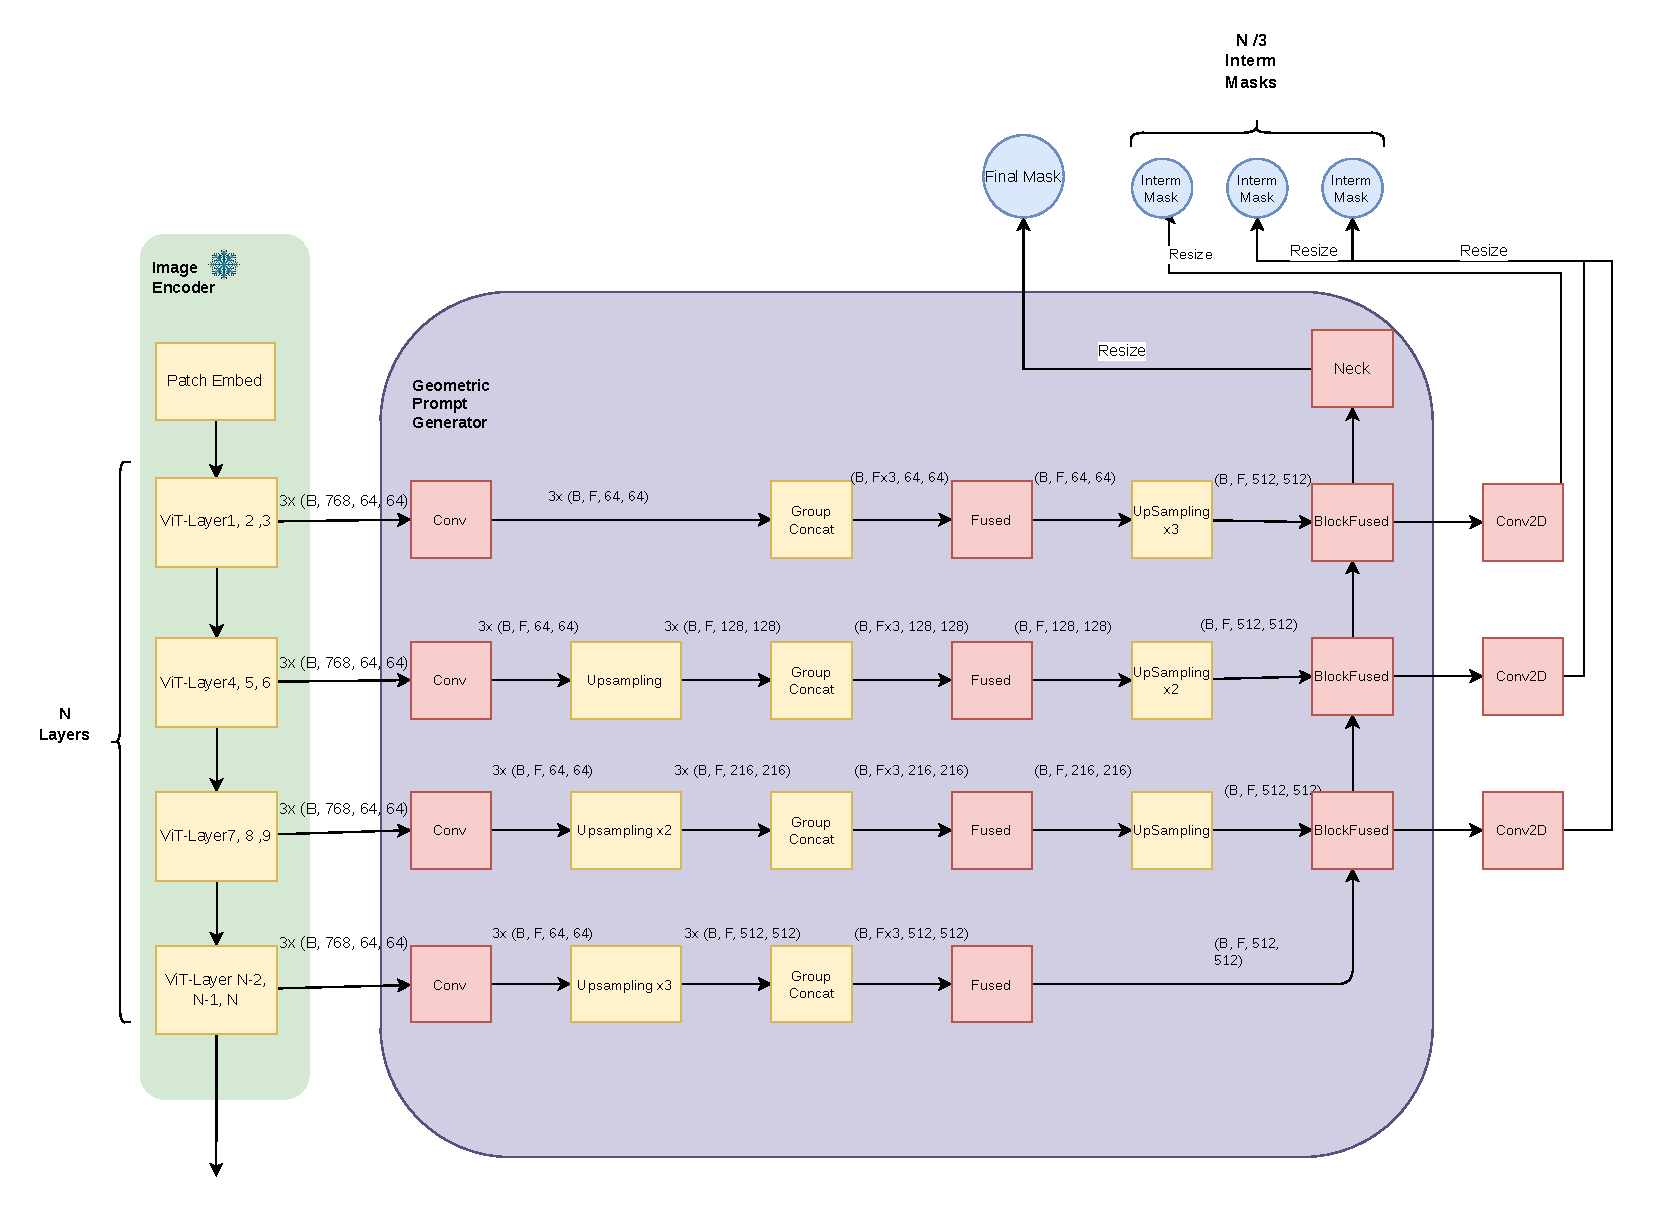
\includegraphics[width=1.2\textwidth]{graphics/approach/prompter.pdf}
    }
    \caption{Multi-scale Fusion Module}
    \label{fig:multiscalefusion}
\end{figure}
% \section{Hyperparameter Optimisation}

\section{Dataset Preparation}
% \subsection*{Data Preprocessing}
% \subsection*{Prompt Preparation}

The Figure \ref{fig:prompt_pipeline} illustrates the overall pipeline of prompt preparation for GAN. This includes creating point prompts, bounding box prompts, and noisy mask prompts for the input adapter in phase 1 as well as creating prompts from auxiliary masks from automatic prompt generator from phase 3.

\begin{figure}[!h]
    \centering
    % 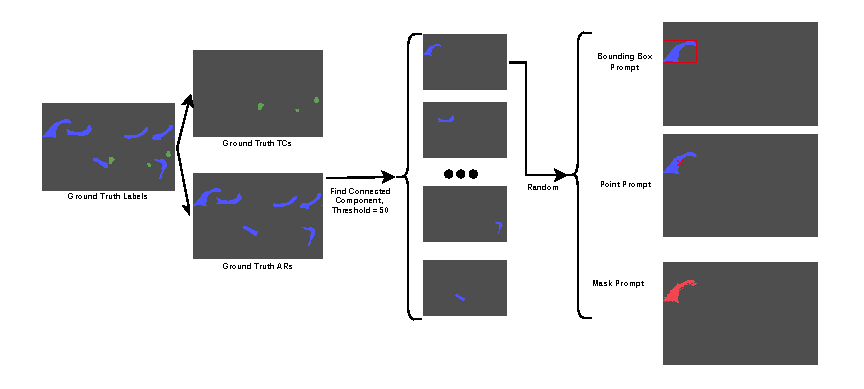
\includegraphics[width=1\textwidth]{graphics/approach/prompt_pipeline-1.pdf}
    \makebox[\textwidth][c]{%
    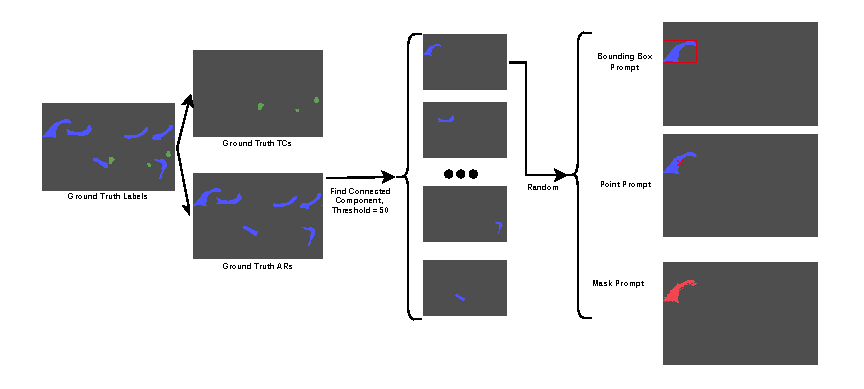
\includegraphics[width=1.2\textwidth]{graphics/approach/prompt_pipeline-1.pdf}
}
    \caption{Prompt Preparation Process}
    \label{fig:prompt_pipeline}
\end{figure}

The Figure \ref{fig:point_prompt_generation} and \ref{fig:noisy_mask_generation} describe the process of creating point prompts and noisy mask prompts in detail. To generate positive point prompts, the binary mask is first processed using an erosion operation with a kernel size determined by the object area. Positive points are then randomly sampled from this eroded region, ensuring the points remain well within the object boundaries. For negative point prompts, the pipeline utilizes two different dilation kernels. A smaller kernel and a big kernel are applied to the mask, and the smaller dilated version is subtracted from the larger one to define a boundary region for sampling negative points. 

\vspace{-2em}
\begin{figure}[!h]
    \centering
    % 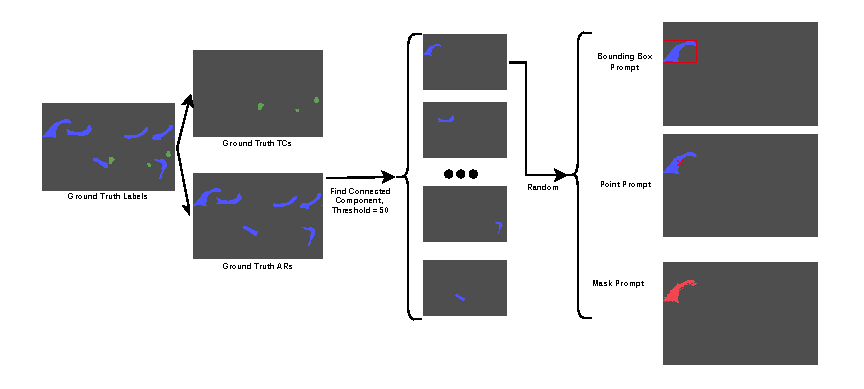
\includegraphics[width=1\textwidth]{graphics/approach/prompt_pipeline-1.pdf}
    \makebox[\textwidth][c]{%
    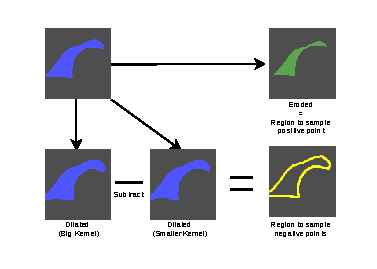
\includegraphics[width=0.7\textwidth]{graphics/approach/point_prompt.pdf}
}
\vspace{-2em}
    \caption{Sampling Negative and Positive Point Prompts}
    \label{fig:point_prompt_generation}
\end{figure}

The noisy mask prompt generation involves a multi-step interpolation and residue calculation process. The input mask is interpolated to a small size and then interpolated back to its original size to create a recovered mask. This recovered version is subtracted from the original input to identify incoherent regions. These regions are thresholded and then combined with Gaussian noise via element\_wise multiplication. Finally, the noise is integrated back into the mask through element\_wise addition to produce a dense, noisy mask prompt.

\vspace{-2em}
\begin{figure}[!h]
    \centering
    % 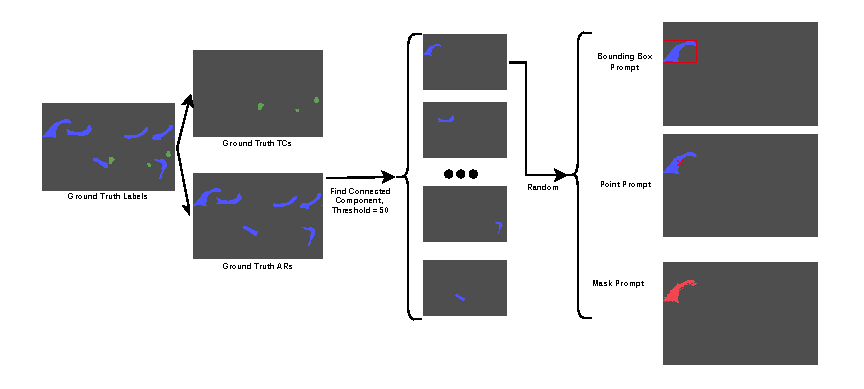
\includegraphics[width=1\textwidth]{graphics/approach/prompt_pipeline-1.pdf}
    \makebox[\textwidth][c]{%
    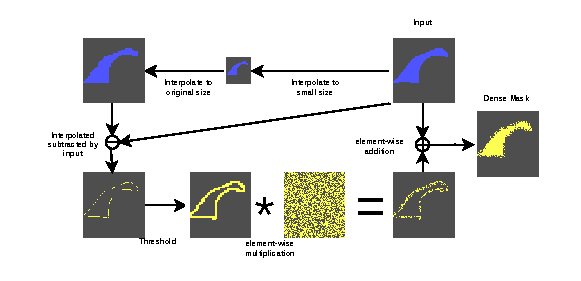
\includegraphics[width=1.2\textwidth]{graphics/approach/noisy_mask.pdf}
}
\vspace{-2em}
    \caption{Create Noisy Mask Prompts}
    \label{fig:noisy_mask_generation}
\end{figure}


% \begin{figure}[!h]
% \centering
% \vspace{-3em} 
% % Top Image
% % \begin{center}
% %     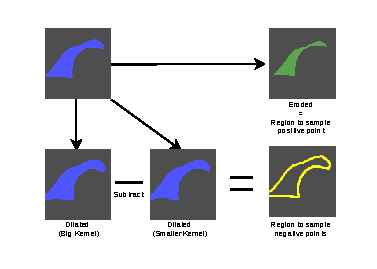
\includegraphics[width=0.7\textwidth]{graphics/approach/point_prompt.pdf}
% %     \caption{Sampling Negative and Positive Point Prompts}
% %     \label{fig:point_prompt_generation}
% % \end{center}
% \vspace{-3em} % Adds a small vertical gap between the two plots
% % Bottom Image
% \begin{center}
%     % \makebox[\textwidth][c]{%
%     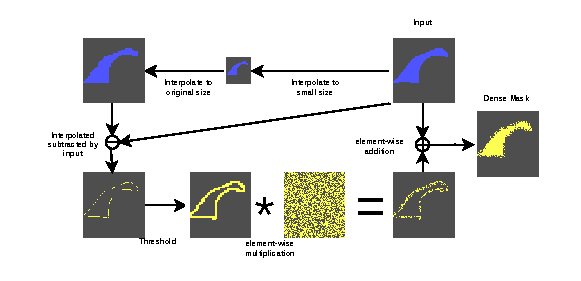
\includegraphics[width=1\textwidth]{graphics/approach/noisy_mask.pdf}
%     \caption{Create Noisy Mask Prompts}
%     \label{fig:noisy_mask_generation}
% \end{center}

% \caption{Prompt Generating Process}


% \end{figure}
\section{Loss Function}
To adapt the Segment Anything Model (SAM) to the unique characteristics of the ClimateNet dataset, a systematic hyperparameter optimization was conducted. The primary goal of this search was to identify the optimal balance between pixel-wise classification accuracy and regional mask overlap, specifically addressing the extreme class imbalance where background pixels constitute approximately 93.9\% of the data.

\subsection*{Search Strategy and Configuration}\label{searchstrat}  

We implemented a random search strategy over 40 iterations to explore the high-dimensional space of the hybrid loss function. To ensure computational efficiency during this search phase, the models were trained on a representative subset consisting of 20\% of the training data. Validation was performed using the ViT-B (Vision Transformer Base) version of the SAM image encoder. 
This methodology is grounded in several practical considerations:

\begin{itemize}
\item Efficiency: Training on a 20\% subset allows for a broader exploration of the parameter space within a fixed compute budget.
\item Generalizability: Because ClimateNet consists of global atmospheric rasters with recurring geophysical patterns, a 20\% subset provides sufficient structural diversity—including circular TC structures and ribbon-like AR corridors—to identify robust hyperparameter trends that generalize to the full dataset.
\item Architecture Consistency: Utilizing the ViT-B backbone ensures that the identified hyperparameters are optimized for the specific feature resolution $(64 \times 64)$ feature grid and embedding space of 256 dimensions used in the final adaptation phase.
\end{itemize}

\begin{table}[h]
\centering
\begin{tblr}{
  colspec = {llXX}, % X column automatically calculates width and wraps text
}
Parameter & Feature & Search Values & Reasons \\ 
\hline
Tversky $(\alpha, \beta)$ & TC & (0.05, 0.95), (0.2, 0.8), (0.3, 0.7), (0.4, 0.6), (0.5, 0.5) & Prioritizes recall for rare circular structures; (0.5, 0.5) serves as the Dice baseline. \\ 
Tversky $(\alpha, \beta)$ & AR & (0.3, 0.7), (0.4, 0.6), (0.5, 0.5), (0.6, 0.4) & Balanced approach for common ribbon forms; (0.5, 0.5) serves as the Dice baseline. \\ 
Focal $(\alpha, \gamma)$ & TC & (0.95, 5), (0.99, 2.5), (0.99, 5), (0.995, 4), (0.995, 6), (0.995, 8), (1, 0) & Combats the 257:1 background to TC ratio; (1, 0) serves as the BCE baseline. \\ 
Focal $(\alpha, \gamma)$ & AR & (0.80, 1), (0.85, 2), (0.85, 5), (0.90, 2), (0.95, 3), (1, 0) & Addresses the 17:1 background to AR ratio; (1, 0) serves as the BCE baseline. \\ 
\hline
\end{tblr}
\caption{Hyperparameter search space for SAM adaptation on ClimateNet.}
\label{tab:searchspace}
\end{table}


\subsection*{Search Space}
The search space was specifically designed to prioritize recall $\beta$ over precision $\alpha$ for TCs, as models tend to miss TC events. To establish a performance baseline against standard, unweighted loss components, the experiments included configurations where Focal loss reduces to standard Binary Cross-Entropy $(\gamma=0, \alpha=1)$ and Tversky loss reduces to the Dice coefficient $(\alpha=\beta=0.5)$. 

To combat the severe 257:1 imbalance of TCs, aggressive weighting was tested using high $\gamma$ values up to 8.0 and extreme Tversky ratios such as 0.05/0.95, forcing the model to focus on the sparse, hard pixels defining TC centers. ARs required more moderate Focal $\gamma$ settings between 1.0 and 5.0 and Tversky ratios closer to parity (standard Dice Loss) due to their less extreme 17:1 imbalance, which helps maintain structural integrity without over-penalizing boundary pixels. Furthermore, while extreme recall settings facilitate localization, moderate values like $\alpha_{tc}=0.3$ were incorporated to test the gradient instability that can occur with extremely aggressive settings during the adaptation phase. Table \ref{tab:searchspace} summarizes the specific hyperparameter combinations. 


\section{Spatial Label Smoothing}\label{spatial_smoothing}

The atmospheric variables within the ClimateNet dataset lack the sharp edges found in natural imagery. Physical phenomena like Tropical Cyclones and Atmospheric Rivers transition gradually into the background space. Rigid binary ground truth masks force the model into making definitive choices on ambiguous boundary pixels. This rigid penalty structure causes the model to memorize specific noise, leading to overfitting for the smaller TC class during later training epochs, as empirically observed. Applying a Gaussian blur to the ground truth masks before calculating the hybrid loss creates a continuous spatial gradient. This smooth gradient acts as a spatial regularizer that aligns more accurately with the physical reality of gradual pressure drop offs. Figures \ref{fig:blur_examples} illustrate the effect of label smoothing with varying kernel sizes and sigma values.


\begin{figure}[!h]
    \centering
    \makebox[\textwidth][c]{%
        \begin{minipage}{1.0\textwidth}
            \centering
            \begin{minipage}{0.48\textwidth}
                \centering
                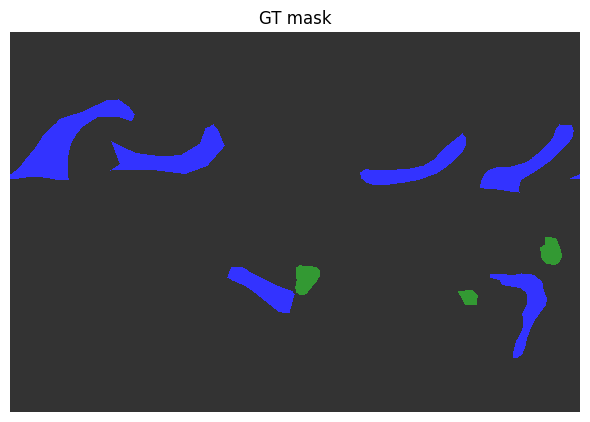
\includegraphics[width=1.05\textwidth]{graphics/approach/blur_0.png}
            \end{minipage}
            \hfill
            \begin{minipage}{0.48\textwidth}
                \centering
                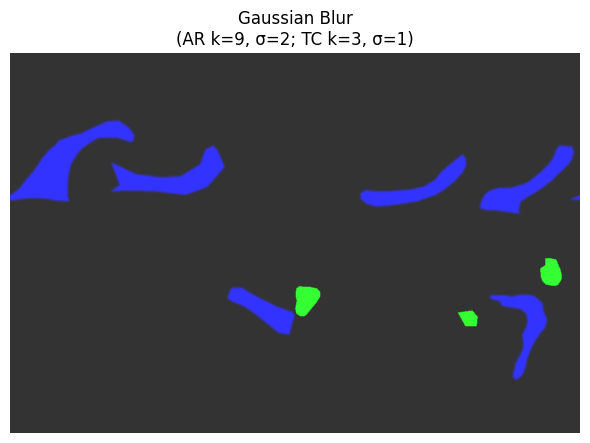
\includegraphics[width=1.05\textwidth]{graphics/approach/blur_1.png}
            \end{minipage}

            % \vspace{0.5cm}

            \begin{minipage}{0.48\textwidth}
                \centering
                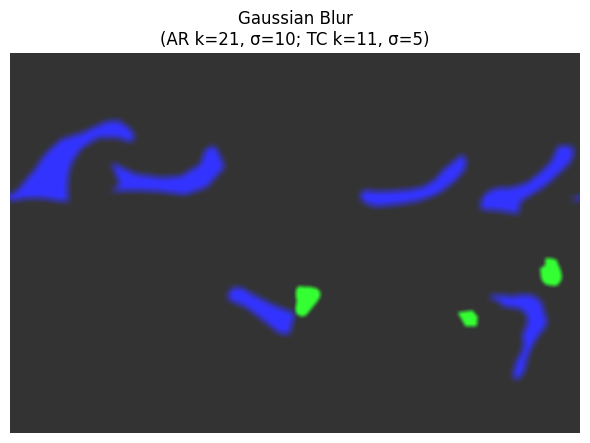
\includegraphics[width=1.05\textwidth]{graphics/approach/blur_2.png}
            \end{minipage}
            \hfill
            \begin{minipage}{0.48\textwidth}
                \centering
                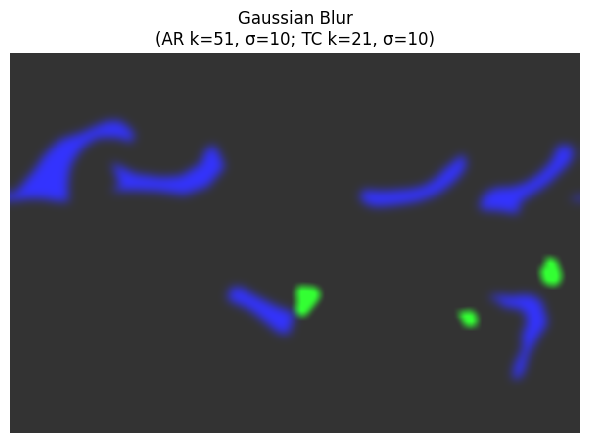
\includegraphics[width=1.05\textwidth]{graphics/approach/blur_3.png}
            \end{minipage}
        \end{minipage}
    }
    \caption{Example of label smoothing with different kernel sizes and sigma values.}
    \label{fig:blur_examples}
\end{figure}


Empirical tests confirm that applying a baseline spatial blur with a kernel size of 3 and sigma of 1.0 for Tropical Cyclones, alongside a kernel size of 9 and sigma of 2.0 for Atmospheric Rivers, successfully mitigates this overfitting behavior and significantly improves performance. Motivated by this success, we establish an independent grid search to identify the optimal blur configuration for each phenomenon. Because TCs and ARs differ drastically in scale, the search space is divided into two independent phases to isolate the effects of the smoothing parameters.

Table \ref{tab:smooth_search} summarizes the hyperparameter search space for the spatial label smoothing. During the search, when the parameters for one class are varied, the parameters for the other class are locked to their respective empirical baseline values to ensure an independent evaluation of the structural boundaries.

\begin{table}[h]
\centering
\begin{tabular}{lll}
Feature & Parameter & Search Values \\
\hline
TC & Kernel Size ($k\_{tc}$) & 3, 11, 21 \\
TC & Sigma ($\sigma\_{tc}$) & 1, 5, 10 \\
AR & Kernel Size ($k\_{ar}$) & 9, 21, 51 \\
AR & Sigma ($\sigma\_{ar}$) & 2, 10, 20 \\
\hline
\end{tabular}
\caption{Hyperparameter search space for spatial label smoothing.}
\label{tab:smooth_search}
\end{table}
\section{Metrics}

\chapter{Result}
\section{Preliminary Result}

\subsection{Hyperparameter Optimisation}

Hyperparameter optimization uses a multi-fidelity approach employed by utilizing a ViT-B encoder and subsampling both the training and validation sets to 20\% of their original size, as described in \autoref{searchstrat}. To assess the effectiveness of each configuration, two primary metrics are reported: Best Max mIoU and Mean Max mIoU. 

The Best Max mIoU represents the absolute peak performance achieved by a single run within a specific parameter group, indicating the model's highest potential under those conditions. Mean Max mIoU averages the peak mIoU across all runs sharing the same parameter setting, serving as an indicator of the setting's reliability and stability. High performance in both metrics suggests a configuration that is not only capable of reaching high accuracy but does so consistently.

The experiments specifically targeted the extreme class imbalance within ClimateNet, where TCs occupy only 0.5\% of the global grid (a 257:1 background-to-foreground ratio) compared to 5.7\% for ARs (a 17:1 ratio).

\subsubsection{Tversky Loss Parameters for Tropical Cyclones}
For the TC class, the search space was biased toward high recall to mitigate the severe imbalance. Experimental results indicate that an $\alpha_{tc}$ of 0.3 paired with a $\beta_{tc}$ of 0.7 yielded the most robust performance, achieving a peak mIoU of 0.3326. Extremely aggressive recall settings, such as an $\alpha_{tc}$ of 0.05, led to training instability and a failure to converge, resulting in a negligible mIoU of 0.0051. 

% This suggests that while recall is a priority for microscopic targets, a moderate alpha-beta trade-off is necessary to maintain gradient stability during the adaptation phase.

\begin{table}[h]
\centering
\begin{tabular}{@{}cccc@{}}
\toprule
$\alpha_{tc}$ & $\beta_{tc}$ & Mean Max IoU TC & Best Max IoU TC\\ \midrule
0.30 & 0.70 & 0.2092 & 0.3326 \\
0.20 & 0.80 & 0.1946 & 0.3096 \\
0.15 & 0.85 & 0.1864 & 0.2001 \\
0.10 & 0.90 & 0.1737 & 0.1970 \\
0.05 & 0.95 & 0.0051 & 0.0051 \\ \bottomrule
\end{tabular}
\caption{Impact of Tversky $\alpha/\beta$ parameters on Tropical Cyclone segmentation.}
\end{table}

\subsubsection{Tversky Loss Parameters for Atmospheric Rivers}
Atmospheric Rivers, characterized by a more moderate 17:1 imbalance ratio, benefited from a more balanced loss configuration. The highest mIoU for the AR class, 0.3028, was achieved with a balanced configuration of $\alpha_{ar}=0.5$ and $\beta_{ar}=0.5$. Unlike the TC class, AR detection does not require extreme recall weighting. 
% The data shows that shifting $\alpha_{ar}$ to 0.4 still maintains high performance (mean mIoU of 0.2392), but the balanced approach provides the most consistent boundary definitions for these larger meteorological structures.

\begin{table}[h]
\centering
\begin{tabular}{@{}cccc@{}}
\toprule
$\alpha_{ar}$ & $\beta_{ar}$ & Mean Max IoU AR& Best Max IoU AR\\ \midrule
0.50 & 0.50 & 0.2387 & 0.3028 \\
0.40 & 0.60 & 0.2392 & 0.2788 \\
0.30 & 0.70 & 0.2190 & 0.2801 \\
0.20 & 0.80 & 0.1902 & 0.1902 \\ \bottomrule
\end{tabular}
\caption{Impact of Tversky $\alpha/\beta$ parameters on Atmospheric River segmentation.}
\end{table}

\subsubsection{Focal Loss Alpha and Gamma for Tropical Cyclones}
The Focal loss configuration for TC prioritized high $\alpha$ and $\gamma$ values to penalize missing difficult targets. A $\gamma_{tc}$ of 5.0 combined with an $\alpha$ of 0.99 provides the optimal focus parameter, providing necessary emphasis on hard boundary pixels. Increasing $\gamma_{tc}$ to 8.0 caused performance to drop to a max mIoU of 0.2714, likely because the loss became overly sensitive to outliers or ground truth noise.


\begin{table}[h]
\centering
\begin{tabular}{@{}cccc@{}}
\toprule
$\alpha_{f\_tc}$ & $\gamma_{tc}$ & Mean Max IoU TC& Best Max IoU TC\\ \midrule
0.990 & 5.0 & 0.2123 & 0.3326 \\
0.990 & 2.0 & 0.2101 & 0.3001 \\
0.995 & 8.0 & 0.1482 & 0.2714 \\ \bottomrule
\end{tabular}
\caption{Performance of Tropical Cyclone detection across Focal Gamma settings.}
\end{table}
As shown in Table \ref{tab:stability_comparison} stable runs maintained a lower average $\gamma_{tc}$ of 2.33. In contrast overfitting runs utilized a higher average $\gamma_{tc}$ of 4.00 which led to an initial peak followed by a drop in performance. These results suggest that while high gamma helps at the beginning of the process it makes the model overly sensitive to specific training samples and reduces generalization. Maintaining $\gamma_{tc}$ between 2.0 and 3.0 is recommended to ensure Tropical Cyclone predictions remain stable until convergence.

\begin{table}[h]
\centering
\begin{tabular}{@{}lcccc@{}}
\toprule
Run Category & Mean $\gamma_{tc}$ & Mean $\alpha_{tc\_tversky}$ \\ \midrule
Stable & 2.33 & 0.30  \\
Overfitting & 4.00 & 0.24 \\ \bottomrule
\end{tabular}
\caption{Comparison of stability metrics between stable and overfitting configurations.}
\label{tab:stability_comparison}
\end{table}

\subsubsection{Focal Loss Alpha and Gamma for Atmospheric Rivers}
For the AR class, a standard $\gamma_{ar}$ of 2.0 outperformed higher focus settings. This setting achieved the peak mIoU of 0.3028. Higher $\gamma$ values, such as 5.0, were less effective for ARs, reducing the peak performance to 0.2652. This confirms that for features with a moderate 17:1 ratio, extreme focal weighting is unnecessary and can potentially hinder the model's ability to learn the general shape of the atmospheric feature.

\begin{table}[h]
\centering
\begin{tabular}{@{}cccc@{}}
\toprule

$\alpha_{f\_ar}$ & $\gamma_{ar}$ & Mean Max IoU AR& Best Max IoU AR\\ \midrule
0.90 & 2.0 & 0.2444 & 0.3028 \\
0.85 & 5.0 & 0.2310 & 0.2652 \\
0.80 & 3.0 & 0.0765 & 0.1902 \\ \bottomrule
\end{tabular}
\caption{Performance of Atmospheric River detection across Focal Gamma settings.}
\end{table}

\subsubsection{Loss Component Weight}
Optimization revealed a numerical imbalance between Focal and Tversky loss components. Initial experiments showed Focal loss values were consistently lower than Tversky components. While heuristics often suggest weighting smaller components for numerical parity, empirical evidence showed this degraded segmentation performance. As shown below, increasing focal weight beyond 10 dropped performance despite achieving comparable loss magnitudes.

\begin{table}[h]
\centering
\begin{tabular}{@{}ccccc@{}}
\toprule
Focal Weight & Mean Focal Loss & Mean Tversky Loss & Max mIoU TC & Max mIoU AR \\ \midrule
1 & 0.03 & 1.98 & 0.3326 & 0.2684 \\
5 & 0.12 & 2.43 & 0.1600 & 0.2198 \\
10 & 0.22 & 2.53 & 0.3410 & 0.2359 \\
20 & 0.25 & 2.69 & 0.2418 & 0.2033 \\
50 & 0.28 & 2.88 & 0.1664 & 0.1572 \\
100 & 0.42 & 3.03 & 0.1334 & 0.1478 \\ \bottomrule
\end{tabular}
\caption{Comparison of loss component magnitudes and resulting segmentation performance across different Focal weights.}
\end{table}

The region\_based Tversky signal primarily drives spatial localization for microscopic targets. High focal weights cause gradients to be dominated by pixel\_wise classification pressures, prematurely biasing the model toward background suppression before Tropical Cyclone structural features are localized. A focal weight of 10 best balances these components, preserving Tversky dominance for structural discovery while allowing Focal loss to refine boundaries.

\subsubsection{Summary of Hyperparameter Optimization Results}

The table below summarizes the optimal parameter settings identified during the random search and their corresponding peak performance metrics.

\begin{table}[h]
\centering
\begin{tabular}{@{}cccc@{}}
\toprule
Metric Category & Parameter & Optimal Value & Peak mIoU \\ \midrule
\textbf{Tversky TC} & $\alpha_{tc} / \beta_{tc}$ & 0.3 / 0.7 & 0.3326 \\
\textbf{Tversky AR} & $\alpha_{ar} / \beta_{ar}$ & 0.5 / 0.5 & 0.3028 \\
\textbf{Focal TC} & $\alpha_{f\_tc} / \gamma_{tc}$ & 0.99 / 5.0 & 0.3326 \\
\textbf{Focal AR} & $\alpha_{f\_ar} / \gamma_{ar}$ & 0.90 / 2.0 & 0.3028 \\
% \textbf{Overall} & Learning Rate & 1e-3 & 0.3326 \\ \bottomrule
\end{tabular}
\caption{Summary of optimal loss hyperparameters for ClimateSAM adaptation.}
\end{table}



\section{Adapt SAM to ClimateNet}
\subsection{Lora}
\subsubsection{Integrating single LoRA component to SAM}
This section presents the performance and parameter efficiency of integrating LoRA into the SAM image encoder. Following the optimal hyperparameters identified in the preliminary results, all experiments were conducted using a learning rate of $1e^{-4}$. The evaluation compares vit\_l and vit\_b backbones across ranks 32 and 64 to determine the impact of model capacity and adaptation rank on segmentation accuracy.

\begin{table}[h]
\centering
\begin{tabular}{lccc}
\hline
Backbone & Rank & IOU AR & IOU TC \\
\hline
vit\_l & 64 & 0.4136 & 0.6005 \\
vit\_l & 32 & 0.4060 & 0.6009 \\
vit\_b & 64 & 0.4387 & 0.6201 \\
vit\_b & 32 & 0.4222 & 0.6020 \\
\hline
\end{tabular}
\caption{LoRA Performance Comparison}
\label{tab:lora_performance}
\end{table}



Table \ref{tab:lora_performance} details the IOU scores for AR and TC. The vit\_b backbone consistently achieves higher accuracy than vit\_l across all configurations. At rank 64, vit\_b reaches an IOU of 0.4387 for AR and 0.6201 for TC, while vit\_l achieves 0.4136 and 0.6005, respectively. For both architectures, increasing the rank from 32 to 64 results in improved IOU scores, particularly for AR detection.

The parameter distribution and training overhead are shown in Table \ref{tab:lora_params_final}. The vit\_l configuration with rank 64 utilizes 14.41M trainable parameters, which represents 4.41\% of the total model. In comparison, the vit\_b configuration with rank 64 uses 10.48M trainable parameters, accounting for 10.06\% of its total architecture. While vit\_l has a larger total parameter count due to its frozen backbone, vit\_b requires fewer absolute trainable parameters and provides superior IOU results.


\begin{table}[h]
\centering
\begin{tabular}{lcccccccc}
\hline
Backbone & Rank & Adapter & Decoder & LoRA & Train & Frozen & Total & \% Train \\
\hline
vit\_l & 64 & 5.2K & 8.12M & 6.29M & 14.41M & 312.34M & 326.75M & 4.41\% \\
vit\_l & 32 & 5.2K & 8.12M & 3.14M & 11.26M & 312.34M & 323.61M & 3.48\% \\
vit\_b & 64 & 5.2K & 8.12M & 2.35M & 10.48M & 93.73M & 104.21M & 10.06\% \\
vit\_b & 32 & 5.2K & 8.12M & 3.14M & 9.30M & 93.73M & 103.03M & 9.03\% \\
\hline
\end{tabular}
\caption{Detailed Parameter Breakdown for LoRA-Adapted SAM}
\label{tab:lora_params_final}
\end{table}

The training dynamics illustrated in Figure \ref{fig:iou_lora_single} provide insights into model generalization and overfitting. While AR validation curves show steady improvement or stabilization, TC curves exhibit significant fluctuations and a decline in performance after an early peak.

For both vit\_b and vit\_l backbones, the TC validation IOU reaches its maximum within the first 10 to 15 epochs before degrading. This behavior suggests the models begin to memorize specific noise in TC training samples rather than learning generalized features. This trend is especially pronounced in vit\_l configurations, which fail to maintain a stable validation IOU despite their larger capacity. The instability in TC curves suggests that its smaller, localized structures are more susceptible to overfitting during LoRA adaptation.

\begin{figure}[!h]
    \centering
    \begin{minipage}[b]{0.45\textwidth}
        \centering
        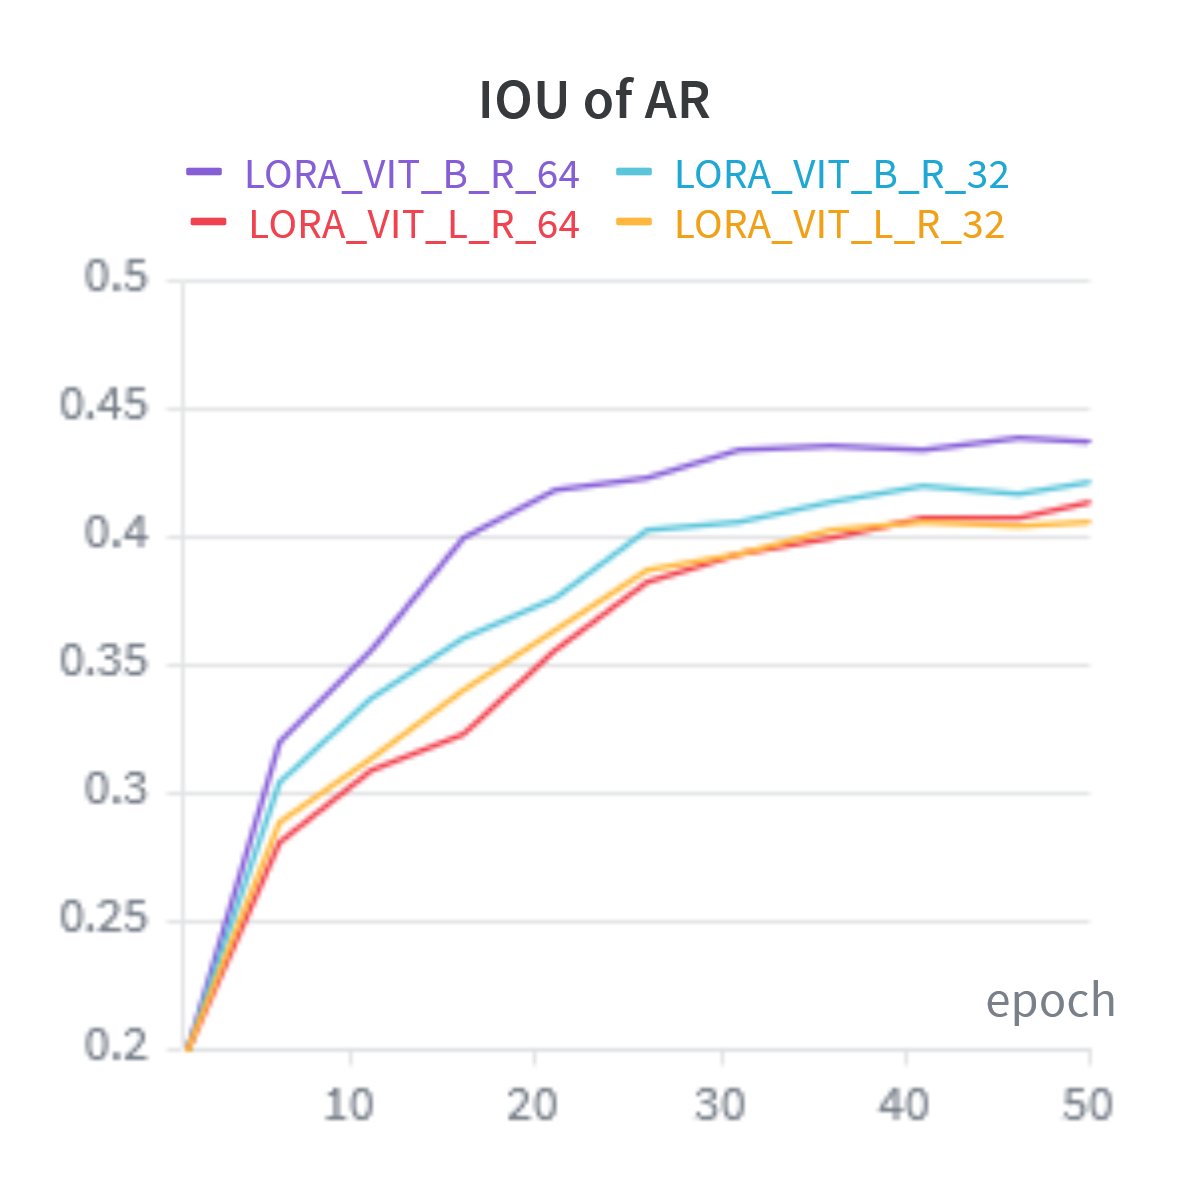
\includegraphics[width=\textwidth]{graphics/result/LORA_SING_AR.png}
        \caption{AR Validation IOU}
    \end{minipage}
    \hfill
    \begin{minipage}[b]{0.45\textwidth}
        \centering
        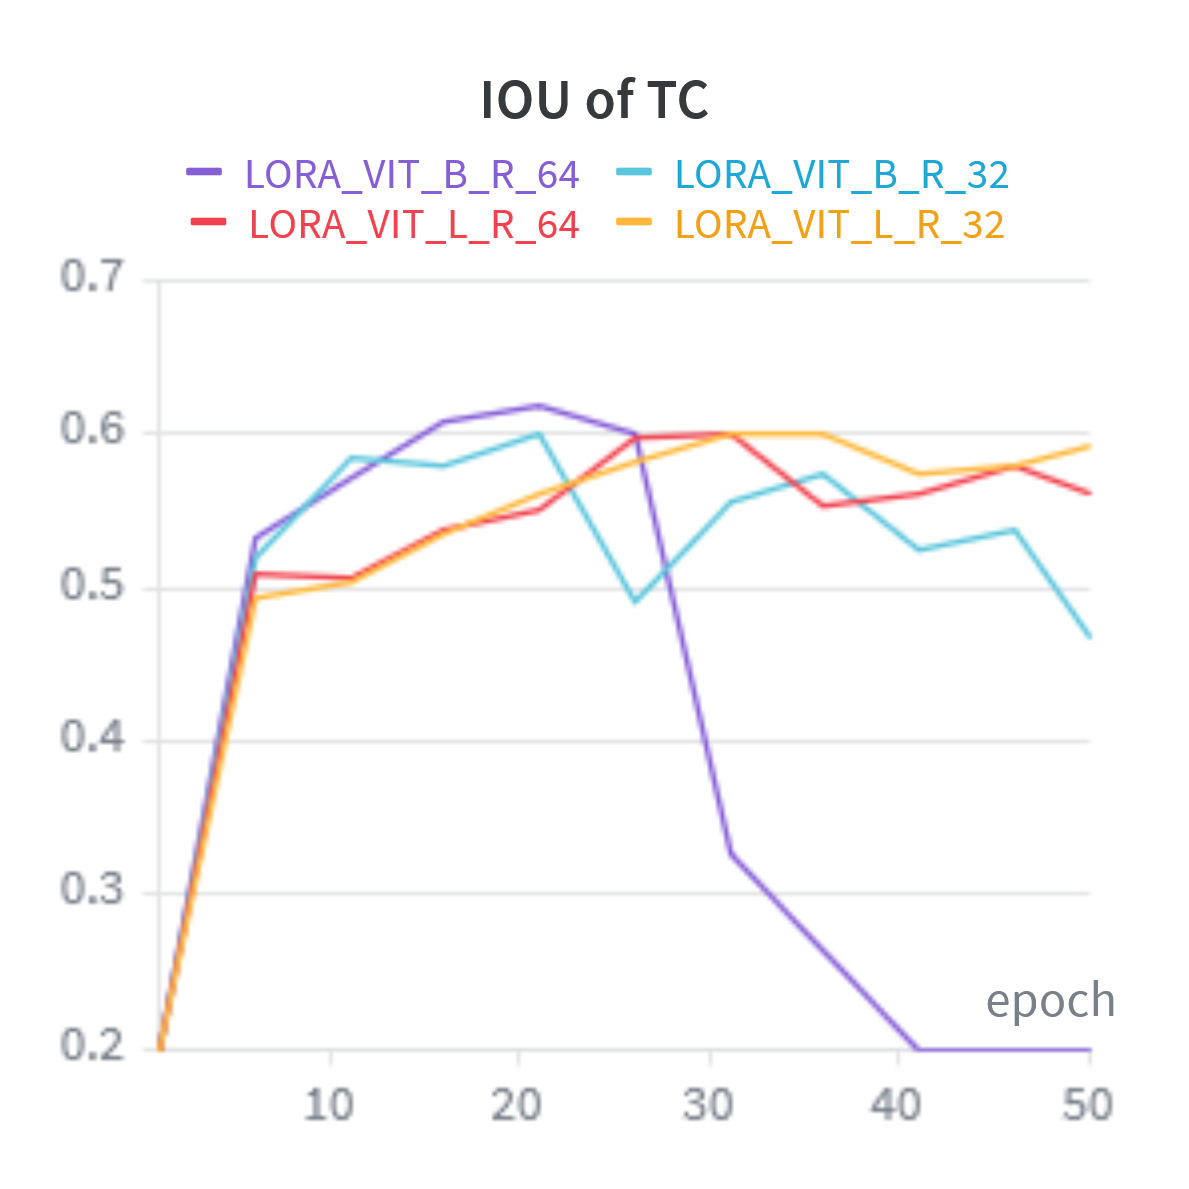
\includegraphics[width=\textwidth]{graphics/result/LORA_SINGLE_TC.png}
        \caption{TC Validation IOU}
    \end{minipage}
    \caption{Validation IOU curves for AR and TC during training}
    \label{fig:iou_lora_single}
\end{figure}
\subsubsection{Integrating single LoRA component to SAM [WITH AUGMENTATION]}
To address TC overfitting, we investigated data augmentation using Horizontal Flip, Vertical Flip, and Random Horizontal Roll ($p=0.5$, shift\_limit$=0.5$). We hypothesized these geometric transforms would be counterproductive as ClimateNet relies on global spatial compositions where geographic orientation is critical. The results in Figure \ref{fig:lora_augmentation} confirm this; while augmentation narrowed the training-validation gap, it hindered effective generalization, causing a sharp mIoU decline for both AR and TC compared to the non-augmented baseline.
\begin{figure}[!h]
    \centering
    \begin{minipage}[b]{0.8\textwidth}
        \centering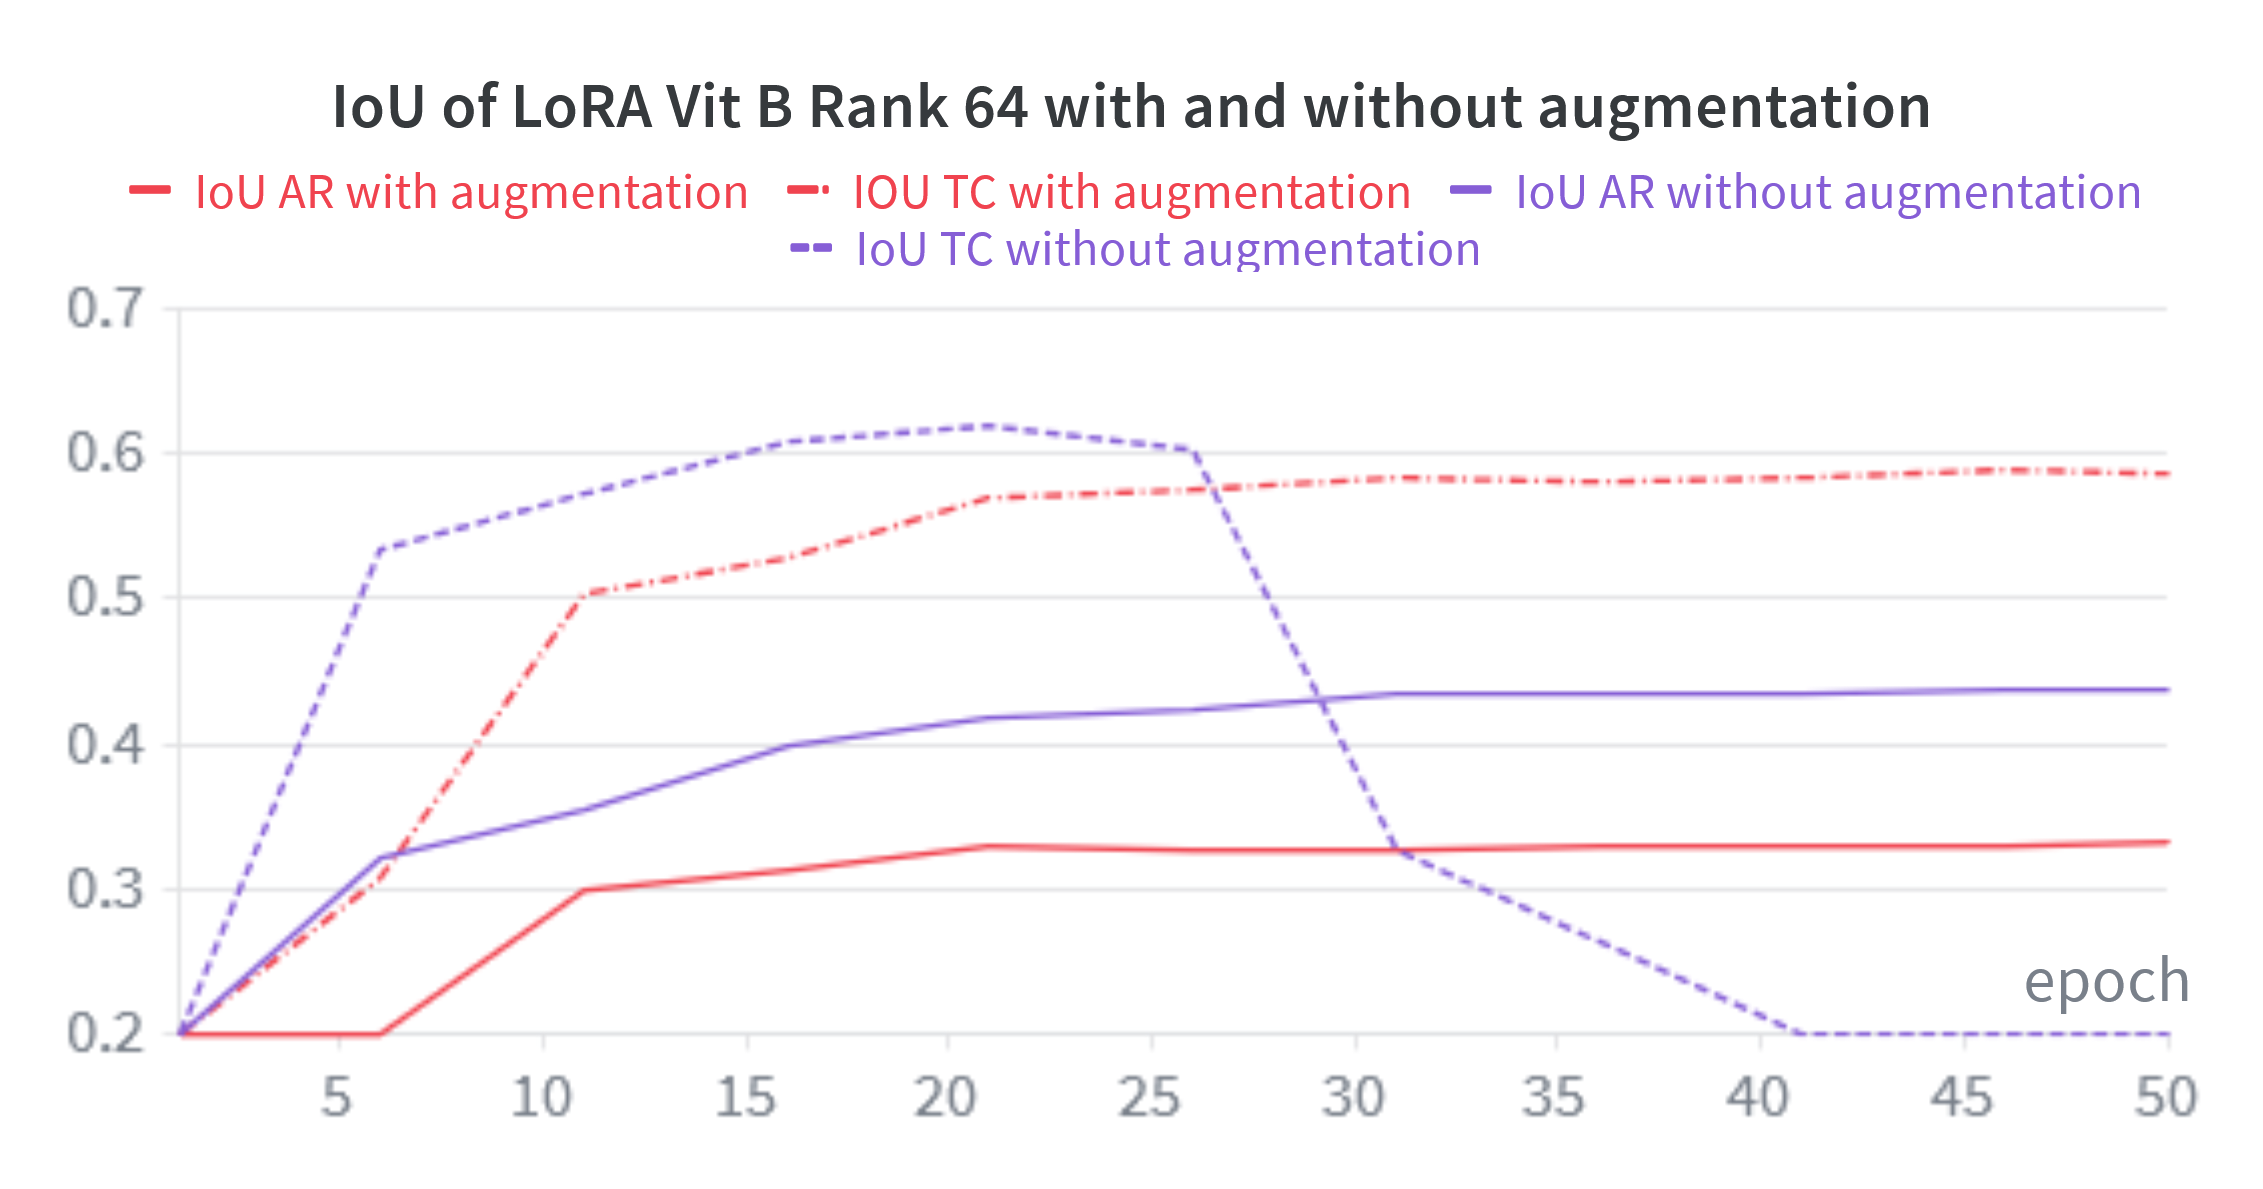
\includegraphics[width=\textwidth]{graphics/result/lora_augmentation.png}
        \caption{Augmentation Performance}
    \end{minipage}
    \caption{Comparison between standard LoRA and augmented training.}
    \label{fig:lora_augmentation}
\end{figure}

\subsubsection{Integrating specialized LoRA components for ARs and TCs}

\subsubsection{SAM with Single infused token}
This section evaluates SAM using a single token prompt strategy. As shown in 
Table \ref{tab:single_token_params}, vit\_b achieves a peak IoU of 0.3771 for 
ARs, while vit\_l performs better on TCs at 0.5694. However, the larger capacity 
of vit\_l introduces significant computational overhead. With 321.74M total 
parameters, it requires approximately 3.23 hours for training compared to the 
2.05 hours needed for the smaller vit\_b architecture.

\begin{table}[h]
\centering
\begin{tabular}{lcccccccc}
\hline
Backbone & IoU AR & IoU TC & Decoder & Encoder & Train & Frozen & Total & \% Train \\
\hline
vit\_l & 0.3015 & 0.5694 & 1.47M & 7.92M & 9.39M & 312.35M & 321.74M & 2.92\% \\
vit\_b & 0.3771 & 0.5292 & 1.07M & 1.58M & 2.65M & 93.74M & 96.40M & 2.75\% \\
\hline
\end{tabular}
\caption{Detailed Parameter Breakdown and Performance for Single Token SAM}
\label{tab:single_token_params}
\end{table}


Training dynamics in Figure \ref{fig:iou_single_token} reveal that the model cannot 
improve ARs and TCs scores at the same time. This inverse relationship 
indicates catastrophic forgetting, where optimization for large scale ARs 
effectively overwrites representations required for localized TCs. The 
single token approach fails to maintain a stable balance across both 
phenomena due to task interference during LoRA adaptation.

\begin{figure}[!h]
    \centering
    \begin{minipage}[b]{0.45\textwidth}
        \centering
        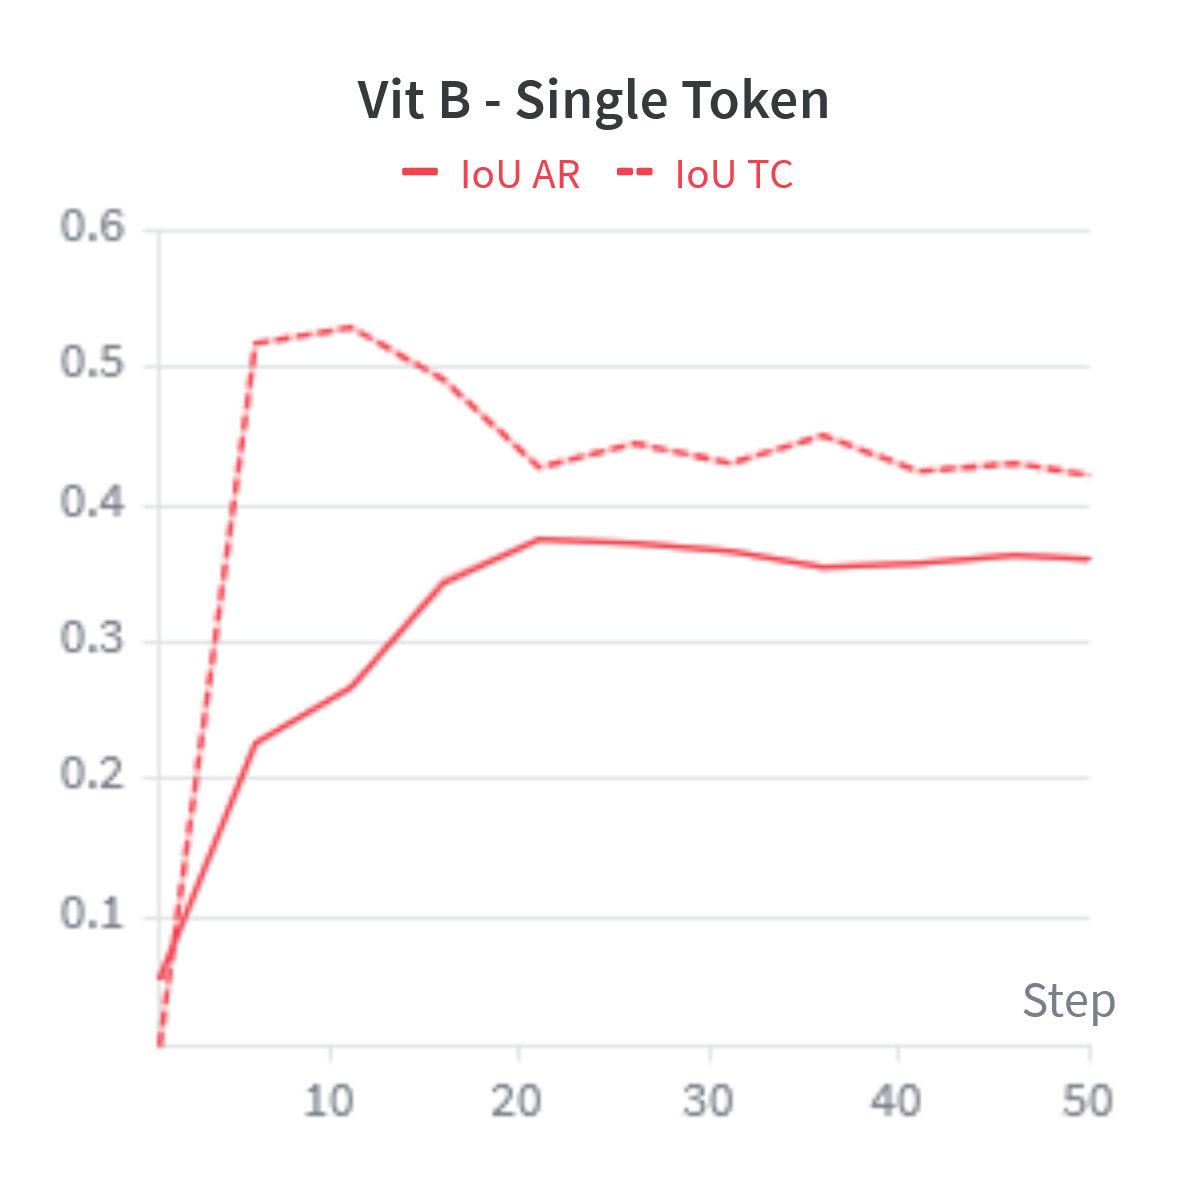
\includegraphics[width=\textwidth]{graphics/result/vitbsingletoken.png}
        % \caption{Vit B}
    \end{minipage}
    \hfill
    \begin{minipage}[b]{0.45\textwidth}
        \centering
        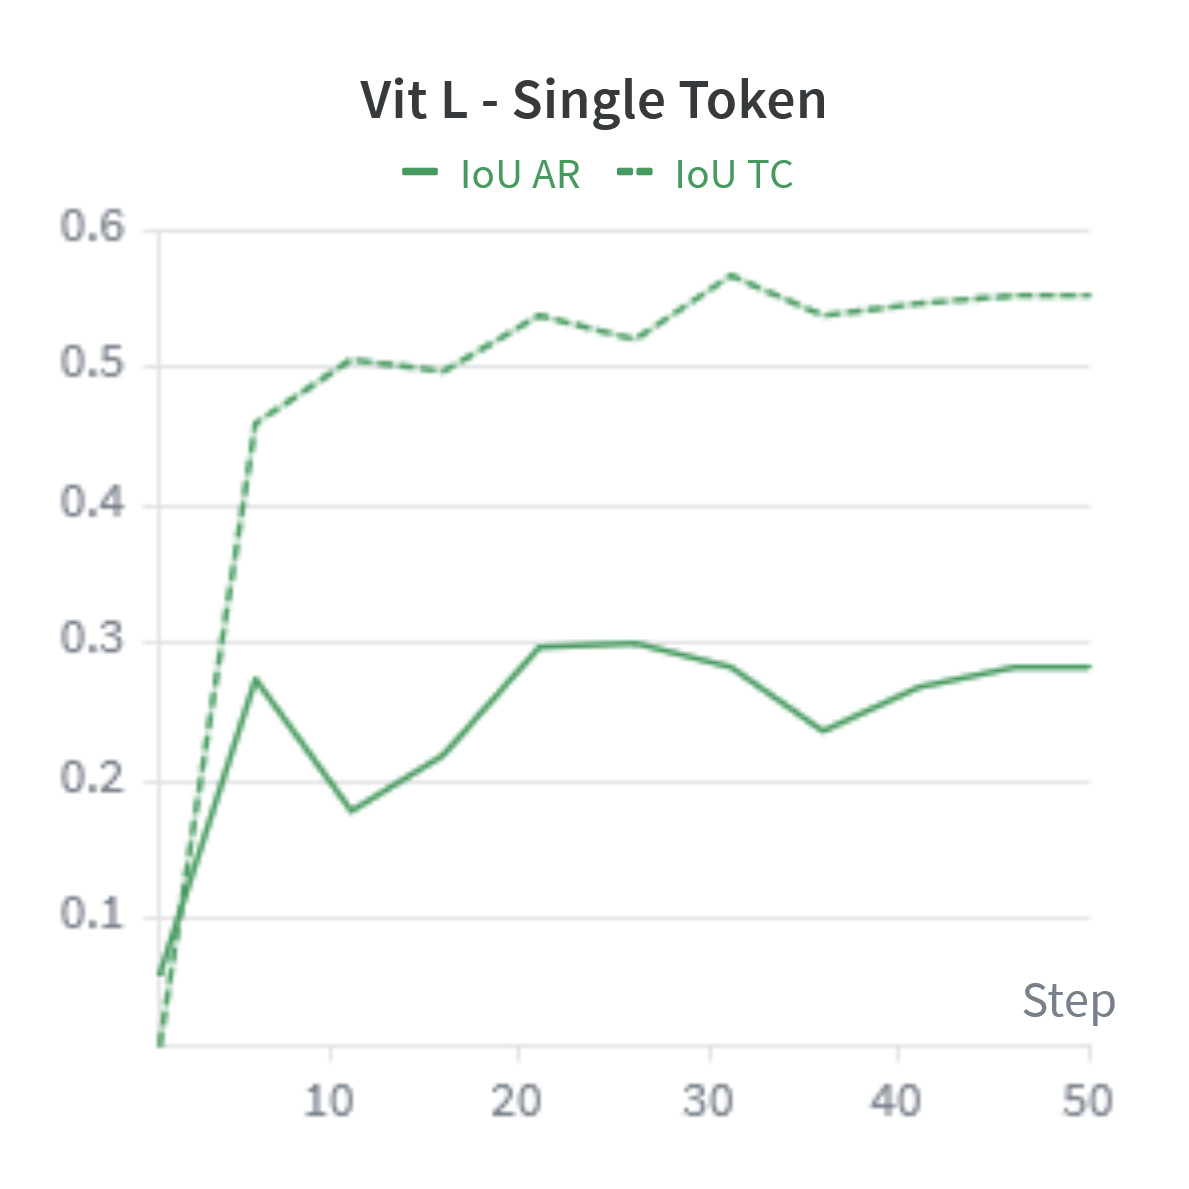
\includegraphics[width=\textwidth]{graphics/result/vitlsingletoken.png}
        % \caption{Vit L}
    \end{minipage}
    \caption{Validation IOU of TCs and ARs curves for SAM with single Token}
    \label{fig:iou_single_token}
\end{figure}




\subsubsection{SAM with Infused Specialized Token}

The training results indicate a positive correlation between the percentage of 
trainable parameters and model performance. As shown in Table 
\ref{tab:infused_token_params}, allocating a higher percentage of trainable 
weights enables the model to capture more complex features, though it increases 
computational demand. For instance, the vit\_l backbone with a 0.75 ratio 
utilizes 4.09\% of the total model (13.33M parameters) and requires 3.42 hours 
to achieve its peak performance. In contrast, the vit\_b backbone at a 0.50 
ratio remains more efficient, utilizing 4.46\% of its architecture (4.38M 
parameters) within 2.15 hours.

\begin{table}[h]
\centering
\begin{tabular}{lccc}
\hline
Backbone & MLP Ratio & IOU ARs & IOU TCs \\
\hline
vit\_l & 0.75 & 0.2426 & 0.5058 \\
vit\_b & 0.75 & 0.2810 & 0.5102 \\
vit\_l & 0.50 & 0.2787 & 0.2973 \\
vit\_b & 0.50 & 0.2867 & 0.5003 \\
\hline
\end{tabular}
\caption{Performance Comparison for Infused Token SAM}
\label{tab:infused_token_perf}
\end{table}

\begin{table}[h]
\centering
\begin{tabular}{lccccccc}
\hline
Backbone & MLP Ratio & Decoder & Encoder & Train & Total & \% Train & Time (h) \\
\hline
vit\_l & 0.75 & 1.47M & 11.86M & 13.33M & 325.68M & 4.09\% & 3.42 \\
vit\_b & 0.75 & 1.21M & 4.74M & 5.95M & 99.69M & 5.97\% & 2.10 \\
vit\_l & 0.50 & 1.47M & 7.92M & 9.39M & 321.74M & 2.92\% & 2.36 \\
vit\_b & 0.50 & 1.21M & 3.17M & 4.38M & 98.12M & 4.46\% & 2.15 \\
\hline
\end{tabular}
\caption{Detailed Parameter Breakdown and Training Duration for Infused Token SAM}
\label{tab:infused_token_params}
\end{table}

Despite the specialization of tokens, the model continues to struggle with catastrophic forgetting, as optimization for large scale ARs structures appears to overwrite the representations required for TCs. This task interference is likely exacerbated by the token integration mechanism; because the tokens are combined via element wise addition and divided by two, the resulting averaging effect may dilute specialized signals and hinder the maintenance of distinct representational boundaries. Consequently, while the larger vit\_l backbone provides increased capacity, the inherent token blending and task interference prevent a stable multi objective balance, leading to the observed decline in TCs performance as the model converges on ARs.


\subsubsection{SAM with Concatenated Specialized Token}

\section{Automatic Prompt Generator for SAM}
\subsection{SAM with CGNet as helper}
\subsection{SAM with multi-scale feature infusion}

\chapter{Discussion}

% % \section{Motivation}
% % \section{Research Questions}
% \chapter{Approach}\label{approach}
% \section{Proposed Model}

\begin{figure}[h]
    \centering
    \includegraphics[width=0.7\textwidth]{graphics/architecture.png}
    \caption{The modular architecture of the proposed \textbf{ClimateSAM} model. The architecture features trainable components—the Input Adapter, Encoder Adapter, and Geometric Prompt Generator—while the core SAM Image Encoder is kept frozen. The Encoder Adapter Architecture architecture incorporates a decoupled design, has separate HQ-prompt tokens, prompt adapters and dedicated MLPs for each task (TC and AR), while the rest of components are shared.}
    \label{fig:climatesam_arch}
\end{figure}

The proposed \textbf{ClimateSAM architecture}, illustrated in Figure \ref{fig:climatesam_arch}, is a modular framework designed for climate pattern segmentation. It begins with an \textbf{Input Adapter} that performs dimensionality reduction, compressing the 16 input climate variables into a 3-channel tensor, analogous to an RGB image. This tensor is then fed into a pre-trained SAM \textbf{Image Encoder}, which remains frozen to leverage its powerful, pre-existing feature extraction capabilities.

To adapt the model to the climate domain, a parameter-efficient \textbf{Encoder Adapter} injects a set of learnable prompt tokens into each transformer layer \cite{xiao2024cat}. To effectively handle the dual-task learning of distinct phenomena (AR vs TC), this adapter is enhanced with two separate, high-quality prompt tokens \cite{ke2023segment}. Each token is managed by a dedicated prompt bridge (a 2-layer MLP), decoupling the learning pathways to mitigate task interference and enable specialized feature adaptation.

An automated \textbf{Geometric Prompt Generator} utilizes intermediate outputs from the vision transformer layers, applying multi-scale fusion and thresholding to dynamically generate point prompts \cite{chen2024sam}. Finally, the \textbf{Mask Decoder} integrates these point prompts, the image features from the encoder, and the task-specific tokens. These tokens are processed through a 3-layer MLP to generate dynamic weights, which are then used to produce the final segmentation masks.

The following sections will explain the choice of the architecture.

\section{Tuning Image Encoder}
We employ prompt tuning, a Parameter-Efficient Tuning (PET) technique, to adapt the heavyweight image encoder of the SAM architecture while keeping its original weights frozen. Drawing from the CAT-SAM-T architecture \cite{xiao2024cat}, we use a decoder-conditioned joint tuning strategy tailored for SAM. This method introduces a set of learnable tokens, alongside the input patch embeddings. CAT-SAM-T introduces a CAT-Token that is mapped to prompt tokens by passing through a prompt bridge (a two-layer MLP), which are later injected into each transformer layer of the image encoder. These, along with the CAT-Token and the weights of the MLP in the mask decoder, are the parameters updated during the adaptation process.

The proposed method operates by keeping the entire pre-trained decoder of the SAM frozen. The learnable CAT-Token is concatenated with SAM's original prompt and output tokens (including mask and IoU tokens). This combined set of tokens serves as the input to the frozen SAM decoder layers. A key aspect of this method is that the updated CAT-Token is independently processed to generate dynamic weights for a new three-layer Multi-Layer Perceptron (MLP). This MLP is subsequently used to generate the refined target masks.

\section{Individual Detection vs Dual Detection}
\begin{figure}[h!]
    \centering
    
    % --- Graphic (a) ---
    % minipage is set to \textwidth, so the two graphics stack vertically
    \begin{minipage}{\textwidth}
        \centering
        % Image (a)
        \includegraphics[width=0.8\textwidth]{graphics/Cat-sam.png}
        
        \vspace{0.2cm} % Small vertical space below the image

        % Manual "Subcaption" (a)
        \centering
        \parbox{0.8\textwidth}{\centering
            \textbf{(a)} Cat-SAM performance on a climate dataset for single detection (TC or AR), utilizing geometric prompts generated from true masks.
        }
        \label{fig:catsam_single}
    \end{minipage}

    \vspace{0.5cm} % Adds vertical space between the two graphics

    % --- Graphic (b) ---
    \begin{minipage}{\textwidth}
        \centering
        % Image (b)
        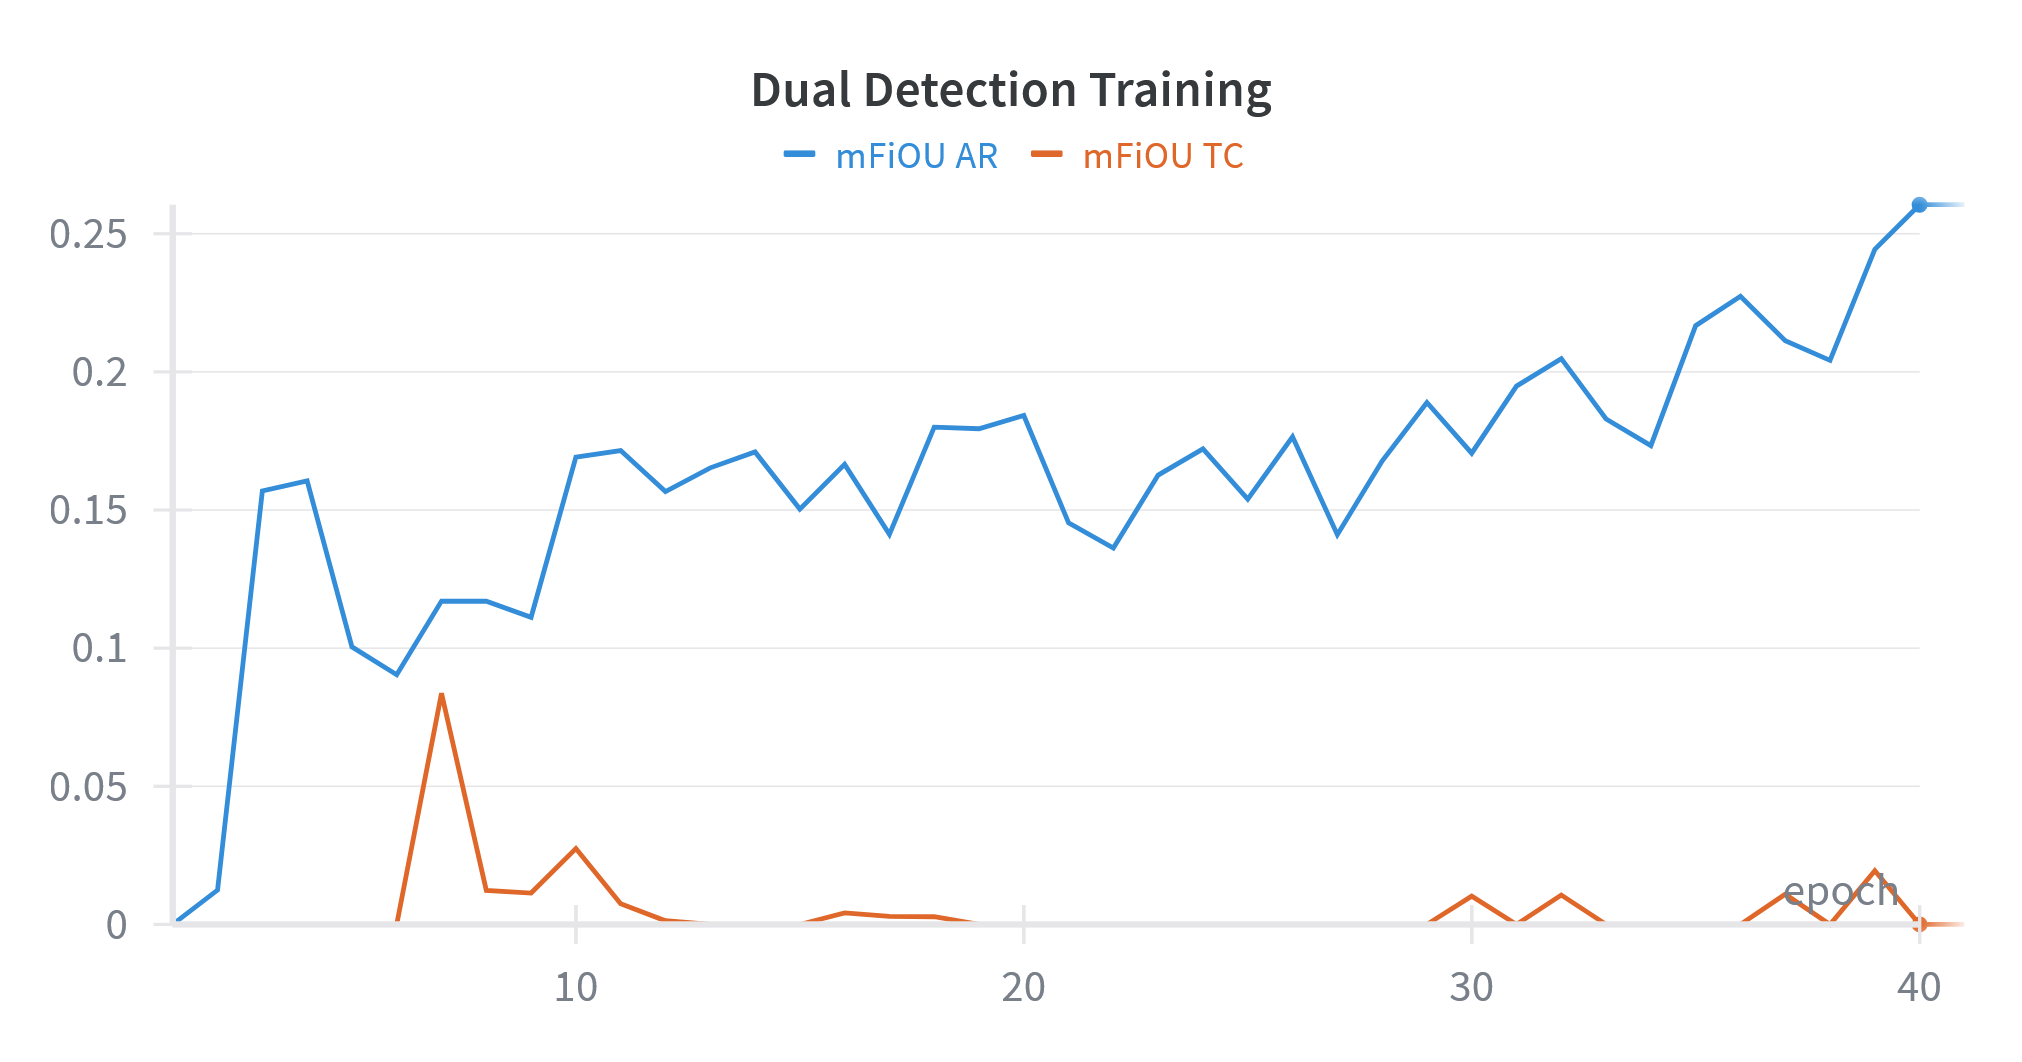
\includegraphics[width=0.8\textwidth]{graphics/dual_long.png}
        
        \vspace{0.2cm} % Small vertical space below the image

        % Manual "Subcaption" (b)
        \centering
        \parbox{0.8\textwidth}{\centering
            \textbf{(b)} Model performance in dual detection using a single shared Encoder Adapter architecture. The model exhibited difficulty in simultaneously learning both Tropical Cyclone (TC) and Atmospheric River (AR) patterns.
        }
        \label{fig:dual_single_adapter}
    \end{minipage}

    % Combined Main Caption
    \caption{Comparison of model performance across single-task and dual-task learning scenarios. (a) shows the high performance achievable when focusing on one climate pattern (Cat-SAM), and (b) illustrates the performance degradation when forcing a single-adapter architecture to learn both TC and AR simultaneously.}
    \label{fig:performance_comparison}
\end{figure}

To empirically validate the performance of the CAT-SAM architecture, the model was evaluated using ground truth geometric prompts derived from annotated labels. The architecture was trained independently on datasets for AR and TC Due to the significant class imbalance, where the spatial extent of TC and AR regions is considerably smaller than the background, the mean Foreground Intersection over Union (mFIoU) was selected as the primary evaluation metric to mitigate potential bias. 

The empirical results demonstrate that CAT-SAM achieves superior performance compared to established baseline models. Specifically, the model attained an mFIoU of 70\% with a comparatively reduced training duration, contingent upon the provision of accurate geometric prompts and a distinct feature training regimen.

To investigate the CAT-SAM model's capacity for dual detection of both AR and TC, we trained the architecture using a multi-class configuration.  This preliminary experiment revealed a significant limitation: the model failed to concurrently improve detection metrics for both phenomena. This outcome suggests the model struggled with the joint feature learning necessary to distinguish between and accurately predict both AR and TC regions simultaneously.

Modified Approach:
To address the issue of learning two different tasks being affected when sharing the same encoder adapter, the modified approach uses two distinct HQ prompt tokens. Each of these tokens has its own prompt bridge (adapters) within the image encoder, and there are two separate 2-layer MLPs, one for each token. This is illustrated in Figure \ref{fig:climatesam_arch} This setup ensures that each task can be learned effectively.

\section{Loss Function}

\begin{table}[h]
    \centering
    \caption{Summary of AR and TC Image and Object Metrics}
    \label{tab:summary_stats}
    % Use p{width} for columns where you need wrapping text.
    \begin{tabular}{llccc}
        \toprule
        \textbf{Type} & \textbf{Statistic} & \thead{\textbf{\#Masks} \\ \textbf{per Image}} & \thead{\textbf{Background/} \\ \textbf{Object Pixel Ratio} \\ \textbf{Per mask}}  & \thead{\textbf{Background/} \\ \textbf{Object Pixel Ratio} \\ \textbf{Per Image} } \\
        \midrule
        \multirow{2}{*}{\textbf{AR}}
            & Mean & 7.43 & 351.36 & 2,242 \\
            & Median & 7.00 & 142.23 & 17 \\
        \midrule
        \multirow{2}{*}{\textbf{TC}}
            & Mean & 2.56 & 880.72 & 149,220 \\
            & Median & 2.00 & 685.37 & 257 \\
        \bottomrule
    \end{tabular}
\end{table}

Table \ref{tab:summary_stats} clearly shows the significant class imbalance in the data. To tackle this, we employ a composite loss function that combines a weighted Binary Cross-Entropy (BCE) loss and a Dice loss. This approach effectively mitigates two primary challenges:
\begin{enumerate}
    \item \textbf{Mask Frequency Discrepancy:} The dataset exhibits a notable difference in the number of masks per data point, with TCs averaging 3.6 masks compared to ARs averaging 0.8.
    \item \textbf{Extreme Foreground-to-Background Pixel Ratio:} The prevalence of background pixels is exceptionally high, with median ratios of 16.98 for ARs and 257.24 for TCs.
\end{enumerate}

Furthermore, empirical observations indicate a tendency for the model to output all-zero masks (predicting only background) due to the vastness of the background. To counteract this, the loss function is specifically formulated to penalize false negatives more heavily than false positives. This is achieved through the weighting mechanisms within both the BCE and Dice loss components, ensuring that the model is strongly incentivized to identify and segment foreground objects, even in the presence of overwhelming background information.

The combined loss is structured as follows:
\begin{align*}
    \text{Loss}_{\text{total}} &= \text{Loss}_{\text{TC}} + \text{Loss}_{\text{AR}} \\
    \text{Loss}_{\text{TC}} &= \text{Loss}_{\text{Dice\_TC}} + \text{Loss}_{\text{BCE\_TC}} \\
    \text{Loss}_{\text{AR}} &= \text{Loss}_{\text{Dice\_AR}} + \text{Loss}_{\text{BCE\_AR}}
\end{align*}


\subsection{Training Pipeline}

\begin{table}[h!]
    \centering
    \caption{Parameter Information for Phase 1 of the Training Scheme.}
    \label{tab:phase1_params} % You should give your table a unique label
    \begin{tabular}{l | l | r}
        \hline
        \textbf{Component} & \textbf{Trainable} & \textbf{Trainable Parameters} \\
        \hline
        \texttt{ORI\_SAM} & False & 0 / 89,677,132 (0.00\%) \\
        \texttt{INPUT\_ADAPT} & False & 0 / 51 (0.00\%) \\
        \texttt{MASK\_DECODER} & True & 1,211,168 / 5,269,508 (22.98\%) \\
        \texttt{IMAGE\_ENCODER} & True & 1,593,344 / 91,264,256 (1.75\%) \\
        \texttt{PROMPT\_ENCODER} & False & 0 / 6,220 (0.00\%) \\
        \hline
    \end{tabular}
\end{table}

The phased training approach is implemented to address computational constraints and facilitate the learning of robust feature representations from input data. This methodology also mitigates parameter forgetting, as a prompt generator's efficacy is contingent upon the model's ability to effectively represent image features.

To enable the tuning of the image adapter and mask decoder in the absence of an automated prompt generator and input adapter, two strategies are employed:

\begin{enumerate}
    \item \textbf{Input Data Normalization:} Following the methodology proposed by Radke \cite{radke2024explaining}, the three most critical parameters for detection—TMQ, U80, and V80—are utilized. These variables are normalized and presented to the model as a three-channel RGB input. This normalization ensures a consistent image distribution for tuning the encoder adapter.
    
    \item \textbf{Geometric Prompt Generation:} For the geometric prompt generators, point and box prompts are derived from the ground truth labels of the objects. The extraction pipeline is detailed in Figure 1. Upon invoking a dataset item, a uniform random decision is made to determine whether point prompts or box prompts will be provided. Point prompts are generated by randomly selecting a pixel coordinate within the object, with a 10\% preference given to centroid points.
\end{enumerate}

The training regimen is conducted on a per-object basis, while validation is performed per image. Given that SAM is designed as an instance segmentation model, per-object training offers a more straightforward supervision mechanism, particularly when prompts are object-specific. Each object is associated with a clear ground truth mask and a defined prompt (either a point or a box). While validation per image assesses if the model can segment all objects accurately in a full image with multiple prompts, evaluated by foreground mIoU. So is the proposed training pipeline:
\begin{itemize}
    \item \textbf{Phase 1:} The Image Adapter and Mask Decoder are trained, while all other components remain frozen. The Table \ref{tab:phase1_params} shows the information of trainable parameters in phase 1.
    \item \textbf{Phase 2:} The Input Adapter is trained, with all other components frozen.
    \item \textbf{Phase 3:} The Prompt Generator is trained, with the Image Adapter and Mask Decoder frozen.
\end{itemize}

\section{Geometric Prompt Generator}


\begin{figure}[h]
    \centering
    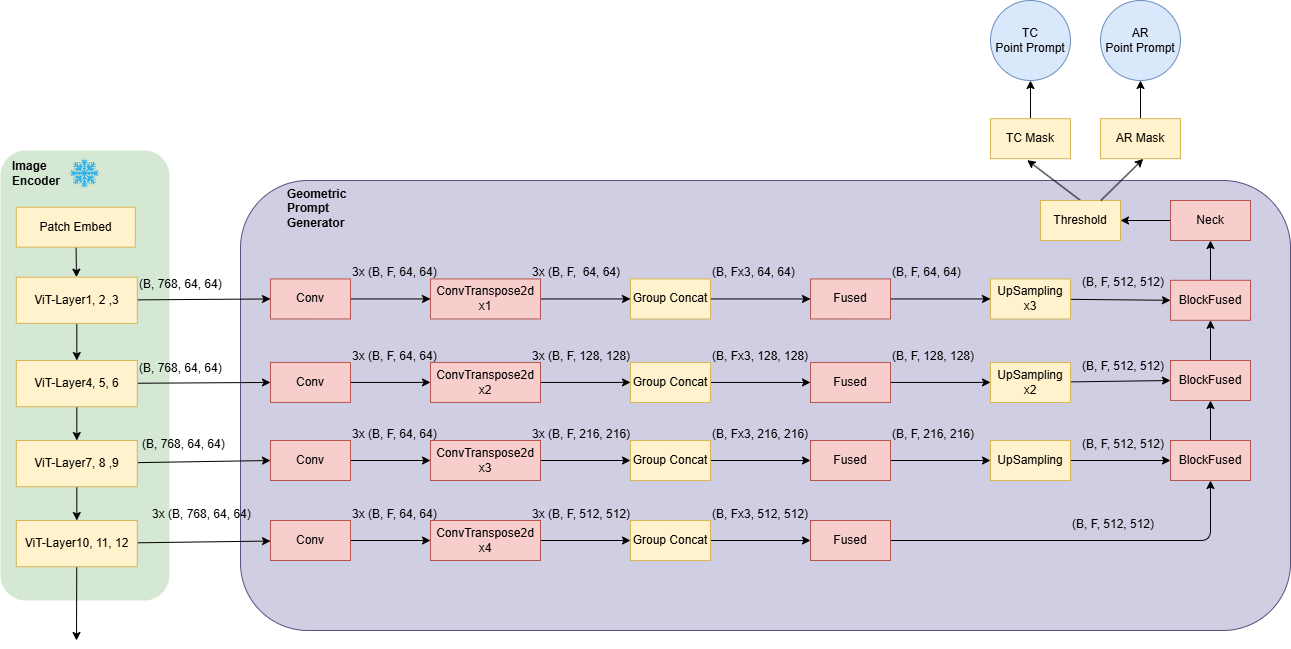
\includegraphics[width=0.9\textwidth]{graphics/prompt.png}
    \caption{Prompt Generator Architecture with mask size of 518}
    \label{fig:prompt_gen}
\end{figure}



The automatic geometric prompt generator is implemented following the completion of Phase 2 training. This sequential approach ensures that the image and mask encoders are sufficiently trained to produce robust feature representations, which are essential for the effective operation of the prompt generator.

The proposed architecture is a multi-scale self-prompt generation mechanism, adapted from the Un-SAM mode \cite{xie2025self, xie2024masksam}. It leverages the intermediate feature maps, from the vision transformer layers. These feature maps are fed into multiple convolutional heads with different strides to produce embeddings at various scales. Subsequently, a Feature Pyramid Network (FPN) integrates these multi-level features via a top-down pathway. Finally, the output from the FPN is passed through a thresholding mechanism to select the final point prompts for segmentation. Figure \ref{fig:prompt_gen} illustrates the architecture.


\begin{enumerate}

    \item \textbf{Channel Reduction and Upsampling:} Each of the three input features per block is first passed through a $1 \times 1$ convolution to reduce the channel dimension from $\text{in\_channels}$ to $\text{fused\_channels}$. These features are then spatially upsampled using a varying number of \textbf{transposed convolutions} ($\texttt{ConvTranspose2d}$), where the degree of upsampling increases with each block index ($n+1$ layers for Block $n$).

    \item \textbf{Group Fusion and Iterative Aggregation:} The three upsampled features are concatenated along the channel dimension ($3 \times \text{fused\_channels}$) and fused via a $1 \times 1$ convolution, followed by a $3 \times 3$ convolution which applies a spatial downsampling (stride 2). For subsequent blocks, the newly fused feature is \textbf{concatenated} with the upsampled output of the previous block, creating an iterative information flow. This combined feature is then upsampled by a factor of 2 using bilinear upsampling ($\texttt{Upsample}$) for the next block.

    \item \textbf{Output Generation:} The final aggregated feature map is passed through a neck layer ($1 \times 1$ Conv) for final channel reduction. This feature then feeds two identical convolutional heads ($\texttt{mask1\_conv}$ and $\texttt{mask2\_conv}$), each using two strided convolutions (with grouped channels in the first layer) to produce the final, single-channel $\texttt{tc\_mask}$ and $\texttt{ar\_mask}$ outputs.

\end{enumerate}

\vspace{-1mm}

\noindent The overall process efficiently aggregates information from multiple encoder stages while iteratively increasing the spatial resolution towards the final mask outputs.


\section{Timeline}
\subsection*{Phase 1: Domain Adaptation Problem Solving (Completed) $\mathbf{\rightarrow}$ Target: 2025-10-15}
Establish the foundational approach and resolve the core domain adaptation challenge.
\begin{itemize}
    \item Literature research.
    \item Solve the domain adaptation problem with the proposed architectural design (Decoupled HQ-Token).
\end{itemize}

\subsection*{Phase 2: Prompt-Free Baseline Generation $\mathbf{\rightarrow}$ 2025-11-15}
Develop a fully prompt-free ClimateSAM as a baseline, without necessarily outperforming results, using an auxiliary network.
\begin{itemize}
    \item Use CGNet for generating auxiliary masks, processing them to give geometric prompts.
    \item Train the input adapter.
\end{itemize}

\subsection*{Phase 3: Prompt Generator Finalization $\mathbf{\rightarrow}$ 2025-12-31}
Integrate intermediate embedding into the prompt generator.
\begin{itemize}
    \item Adapt the current architecture to leverage image encoding to generate a Confidence Map (MAP), which subsequently informs an Adaptive Sampling and Filtering Component. This component will be inspired by the principles of AoP-SAM and SAM-SP \cite{chen2025aop, zhou2024sam}.
    \item Modify the current architecture to incorporate immediate embeddings derived from Vision Transformer (ViT) layers, as to create a multi-scale prompt generator, inspired by Un-SAM and MaskSAM \cite{xie2025self, xie2024masksam}.
\end{itemize}

\subsection*{Phase 4: Optimization and Validation $\mathbf{\rightarrow}$ 2026-01-31}
Refine the system's efficiency and other experiments.
\begin{itemize}
    \item Rescale the proposed architecture to significantly reduce computational resource consumption.
    \item Experimentally evaluate the impact of various augmentations and different hyperparameters on model performance.
    \item Experiment the performance of LoRA vs current prompt token approach.
    \item Systematically perform hyperparameter tuning to maximize model efficacy.
\end{itemize}


\subsection*{Phase 5: Documentation and Submission $\mathbf{\rightarrow}$ 2026-02-28}
Finalize the academic documentation and complete the thesis submission process.
\begin{itemize}
    \item Thesis Writing: Compose and refine the final thesis document.
    \item Submission: Complete the formal submission of the thesis.
\end{itemize}


\chapter{Preliminary Result}
In preliminary training, the proposed model, after completing phases 1 and 2 (with given perfect geometric prompts from true masks), significantly surpassed the baseline performance. This training incorporated three augmentation techniques: horizontal flipping, vertical flipping, and horizontal cyclic shifting, the prompt types in training are chosen randomly point, bounding box, or mask. The prompt types for validation is chosen randomly between point and bounding box.

\begin{table}[h!]
    \centering
    \caption{Segmentation Performance Metrics for Climate Events}
    \label{tab:climate_sam_metrics}
    \begin{tabular}{lccc}
        \toprule
        Category & mIoU & mIoU (w/ Background) & Mean Accuracy \\
        \midrule
        Atmospheric Rivers (ARs) & $0.5084$ & $0.7351$ & $0.8289$ \\
        Tropical Cyclones (TCs) & $0.6095$ & $0.8035$ & $0.8435$ \\
        \bottomrule
    \end{tabular}
\end{table}

\begin{figure}[h!]
    \centering
    
    % First Row (a) and (b)
    \begin{minipage}[t]{0.49\textwidth} % Adjust width to 49% for spacing
        \centering
        % Image (a)
        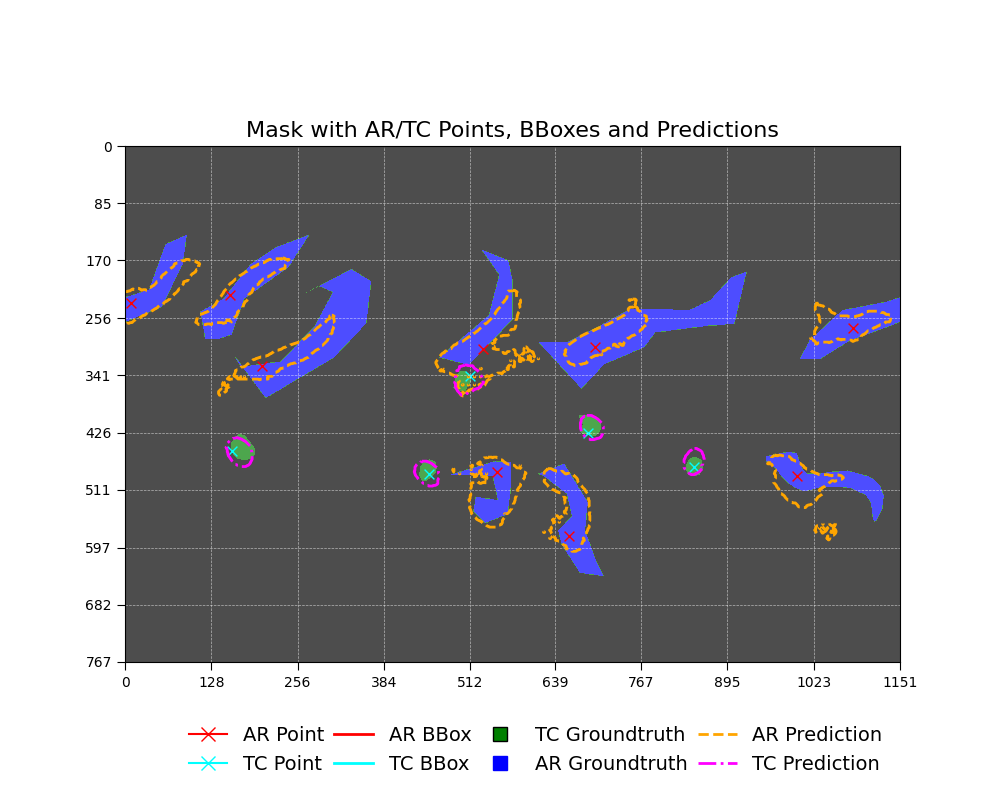
\includegraphics[width=\textwidth]{graphics/valid_1.png} % Image uses full minipage width
        
        \vspace{0.2cm}

        % Subcaption (a)
        \parbox{\textwidth}{\centering
            \textbf{(a)} 
        }
        \label{fig:valid_1}
    \end{minipage}
    \hfill % Horizontal space between minipages
    \begin{minipage}[t]{0.49\textwidth}
        \centering
        % Image (b)
        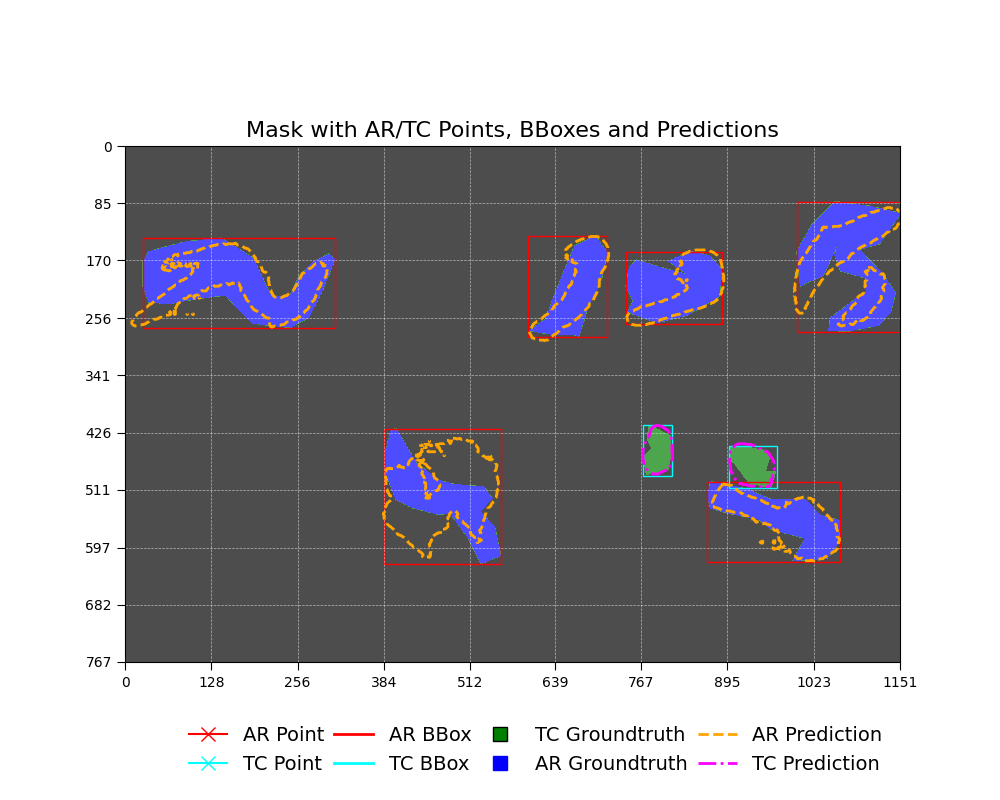
\includegraphics[width=\textwidth]{graphics/valid_2.png}
        
        \vspace{0.2cm}

        % Subcaption (b)
        \parbox{\textwidth}{\centering
            \textbf{(b)} 
        }
        \label{fig:valid_2}
    \end{minipage}

    \vspace{0.5cm} % Vertical space between rows

    % Second Row (c) and (d)
    \begin{minipage}[t]{0.49\textwidth}
        \centering
        % Image (c)
        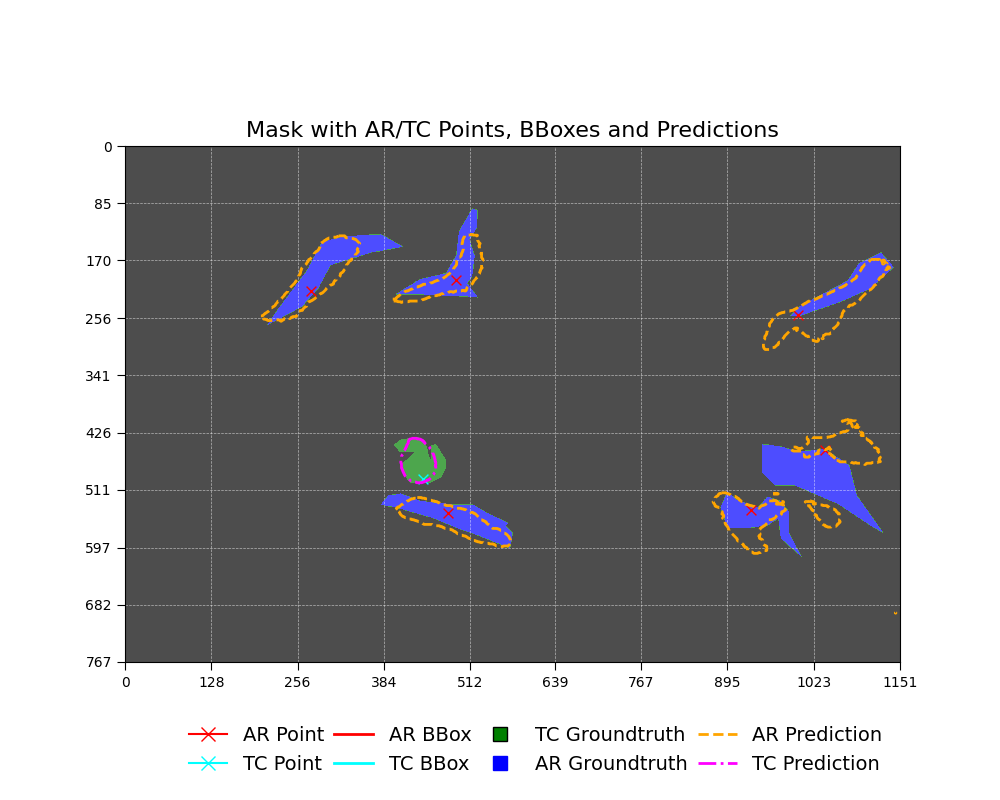
\includegraphics[width=\textwidth]{graphics/valid_3.png}
        
        \vspace{0.2cm}

        % Subcaption (c)
        \parbox{\textwidth}{\centering
            \textbf{(c)} 
        }
        \label{fig:valid_3}
    \end{minipage}
    \hfill
    \begin{minipage}[t]{0.49\textwidth}
        \centering
        % Image (d)
        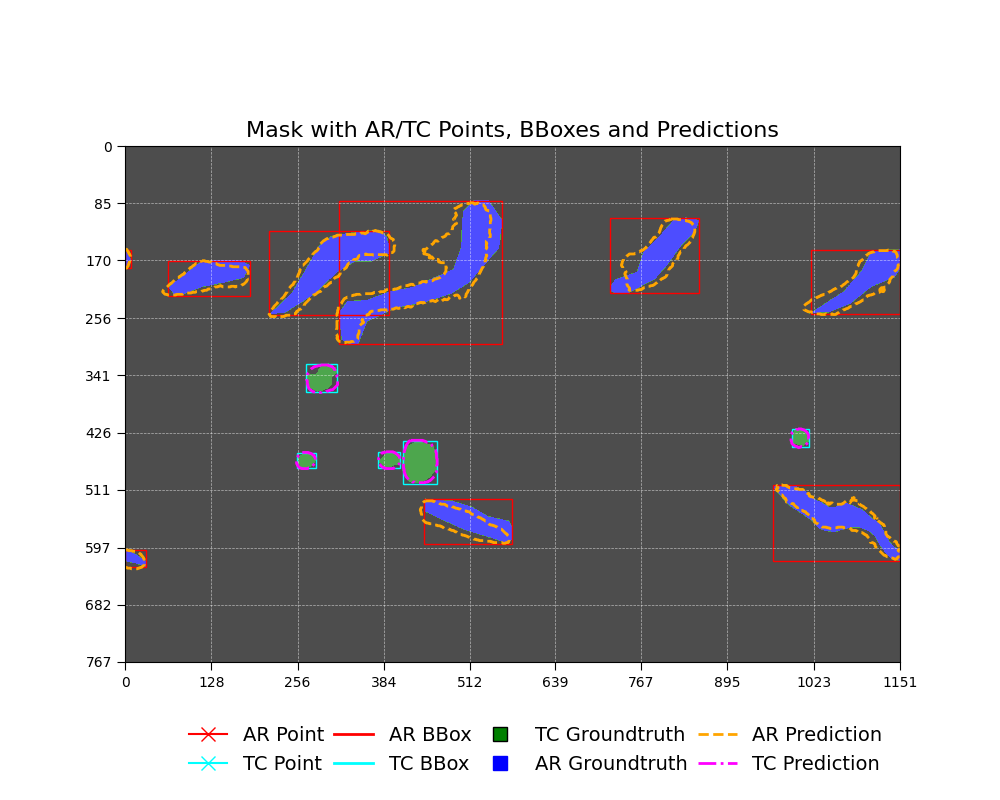
\includegraphics[width=\textwidth]{graphics/valid_4.png}
        
        \vspace{0.2cm}

        % Subcaption (d)
        \parbox{\textwidth}{\centering
            \textbf{(d)} 
        }
        \label{fig:valid_4}
    \end{minipage}

    % Combined Main Caption
    \caption{Valid image at end of training phase for 4 valid examples.}
    \label{fig:valid_examples}
\end{figure}



% \section{Implementation plan and schedules}
% \chapter{}

% 1. Topic introduction:

% The automated detection and tracking of two-dimensional (2-D) and three-dimensional (3-D) atmospheric features, such as cyclones, fronts, jet streams, and atmospheric rivers (ARs), in both simulation and observational data, has become integral to meteorology. These automated techniques find applications in weather forecasting, statistical and climatological studies, and visual data analysis.

% Traditionally, atmospheric features have been detected using physical and mathematical rules. Cyclones, for example, are identified through minima or maxima in variables like sea level pressure and lower-tropospheric vorticity, while fronts are detected via derivatives of thermal variables and threshold-based filters. Atmospheric rivers are identified based on thresholds in integrated water vapor transport. 



% motivation: why detecting tropical cyclone and atmospherical rivers important. (3 Sentences - with references)  traditionally how it was doned. Then there was  an interface and describe how climate scientist do it by hand and costs many hours.



% Example:
% The automated detection and tracking of 2-D and 3-D atmospheric features including cyclones, fronts, jet streams, or atmospheric rivers (ARs) in simulation and observation data has multiple applications in meteorology. For example, automatically detected features are used for weather forecasting (e.g., Hewson and Titley, 2010; Mittermaier et al., 2016; Hengstebeck et al., 2018), statistical and climatological studies (e.g., Dawe and Austin, 2012; Pena-Ortiz et al., 2013;
% Schemm et al., 2015; Sprenger et al., 2017; Lawrence and Manney, 2018), and visual data analysis (e.g., Rautenhaus et al., 2018; Bösiger et al., 2022; Beckert et al., 2023). Features are typically detected based on a set of physical and mathematical rules. For example, cyclones can be identified by searching for minima or maxima in variables including mean 
% sea level pressure and lower-tropospheric vorticity (Neu et
% al., 2013; Bourdin et al., 2022). Atmospheric fronts can be
% identified by means of derivatives of a thermal variable combined with threshold-based filters (Jenkner et al., 2010; Hewson and Titley, 2010; Beckert et al., 2023) and ARs based on thresholding and geometric requirements (Guan and Waliser,
% 2015; Shields et al., 2018).


% Then there is machine learning approach, startrted 

% the manual works in reading 





% 1. Short Motivation. (half page)
% 2. Related Works.
% - SAM
% - CAT-SAM
% - SOS
% - Tim Radke Work: 

% approach:


% Mask prompts:


% - Using a U-NET for dimension reductions.
% - 
